% !TeX root = ../../book.tex
\chapter[集合]{集合:数学的基石}\label{ch:chapter03}

% !TeX root = ../../../book.tex
\section{引言}

现在是时候学习集合了!这部分内容出现在上一章之后,似乎是一个奇怪的跳跃。请详细我们,这是自然且必要的。我们在数学中所做的一切都建立在集合的基础上,所以我们最好现在就开始学习集合并习惯使用集合。

% !TeX root = ../../../book.tex
\subsection{目标}

以下简短内容将向你展示本章如何融入本书的体系。这部分内容会描述我们之前的工作将如何发挥作用,还会激发我们为什么要研究本章出现的主题,并告诉你我们的目标,以及你在阅读时应该记住什么来实现这些目标。现在,我们将通过一系列陈述为你总结本章的主要目标,以及本章结束时你应该获得的技能和知识。以下各节将更详细地重申这些想法,但这里将为你提供一个简短的列表以供将来参考。当学完本章后,请返回此列表,看看你是否理解所有这些目标。你明白为什么我们在这里概述它们很重要吗?你能定义我们使用的所有术语吗?你能应用我们描述的技术吗?

\textbf{学完本章后,你应该能够……}

\begin{itemize}
    \item 定义什么是集合,并给出几个常见的例子。
    \item 使用正确的符号来定义集合并引用其元素。
    \item 定义并描述常见集合操作;即用两个或多个集合创建新集合的方法。
    \item 描述如何比较两组两个集合,并应用恰当的技术来证明此类观点。
    \item 解释自然数与集合的关系,并将其与数学归纳法联系起来。
\end{itemize}


% !TeX root = ../../../book.tex
\subsection{承上}

我们正在构建数学归纳法的正式表述,并将其证明为\emph{定理}。为了实现这一目标,我们需要一些基本对象以便于逻辑严谨地处理和讨论。集合就是那些对象!从历史上看,数学是在二十世纪初才建立在\emph{集合论}的基础之上。在那之前,数学家们倾向于对他们工作背后真正发生的事情``撒手不管''。他们做出了很多``直觉上的''假设,但从未尝试严格且\emph{公理化地}描述他们所做的一切。数学家\textbf{乔治·康托尔(Georg Cantor)}的工作向大家展示了一些令人惊讶且反直觉的结果,这些结果完全正确且与我们的假设一致……于是,我们意识到我们有必要确定我们一直谈论的内容。当然,这并不是要抹黑 1900 年之前的数学家的工作!我们只是说他们一直在玩一个游戏,但并没有真正就一套规则达成一致。这就是集合论\textbf{公理体系}。


% !TeX root = ../../../book.tex
\subsection{启下}

我们的核心动机是不断学习\textbf{证明},理解其本质与运作方式,特别是严谨的数学归纳法。更广泛地说,我们对数学家的实际工作充满兴趣。我们确信,任何数学家都会强调\textbf{集合}在其研究中的重要性。他们或许会表示自己不愿从事纯\emph{集合论}工作,但无人能否认集合的基础地位。

后续所有讨论都将涉及对特定对象集合的陈述。我们将尝试断言(并证明)某些对象具有特定性质。定义这些对象需要集合语言,而表述这些断言则需要数学逻辑——这是我们即将学习的内容。当前首要任务是掌握各类数学对象的表达方式,方能对其进行准确描述。


% !TeX root = ../../../book.tex
\subsection{忠告}

本章将引入若干新颖的数学概念,不同于前两章专注于数字、代数、算术及批判性思维的谜题。这些新思想需要专注阅读并积极思考。学习概念与结论时,请仔细研读并深入反思。数学文本比报刊文章对读者要求更高:它期待你\emph{全神贯注},斟酌每句话的含义,必要时暂停数分钟以确保真正理解。请谨记:阅读数学虽有挑战,但这很正常!不必气馁,将每句话视为整体拼图的关键部分。

若本章的研读时间(含课堂学习时间)等同甚至超过前两章的总和,这不足为奇。根据我们长期以来的观察,最具挑战的往往是集合的\textbf{表示法}。这可能是你首次被要求如此\textbf{精确}而\textbf{严谨}地书写。仅``思路正确''是不够的;我们必须确保文字准确反映思想。完成问题或作业后,请反复检查并自问:``此表述是否合理?是否准确传达了我的本意?读者能否据此理解我的思想?''

此外,本章涉及比常规数学课程更\textbf{抽象}的思维。无论你是否感到吃力,都不可能速读求成。此时更需投入时间消化:精读几页后,在用餐、散步等日常活动中反复思考;寻找现实中的实例;与同伴探讨集合概念。这或许看似多余,但终将使你获益匪浅。请相信我们的经验。


\newpage
% !TeX root = ../../book.tex
\section{``集合''思想}

\subsubsection*{``物以类聚''}

集合的直观概念对你来说可能并不陌生。如果你奥特曼卡收藏者\footnote{原作这里用的是``棒球明星卡'',考虑到中国读者对棒球运动的陌生,译者将其改成风靡中国(青少年界)的奥特曼卡。--- 译者注},拥有``全套''卡片意味着拥有发行商发行的某个系列的每一张卡。如果你和朋友一起玩桌游,你们会在玩之前商定一套``规则'',这样以后就不会出现未解决的争议。如果你在生物、化学或物理课上进行了实验室实验,你会将数据收集到``数据集''中并分析这些结果以检验假设。

这是三种不同情况,每种情况都涉及单词``集或套''(\textbf{set}),那么该单词是如何关联上下文并赋予正确含义的呢?本质上,集合是指基于某些共同属性而组织在一起的对象的全体。在第一个示例中,稀有度为 UR 的每一张卡都属于该特定集合。在第二个示例中,任何商定好的规则都将属于规则集合。在第三个示例中,实验中收集的任何数据都属于该数据集。在每种情况下,都有一个共同的属性,让我们可以将特定对象彼此关联起来,并将它们作为一个集合来引用。

\subsubsection*{数学中的集合}

集合在数学中非常常见、非常流行、同时也非常有用、非常基础。因为数学家研究的是抽象对象以及这些对象之间的关系,因此如果无法引用一组数学对象,就很难准确描述所思考的内容。事实上,我们已经不自觉地用到了集合!

例如,在研究多项式和二次函数求根公式时,我们提到具有负判别式(当 $\frac{b^2}{4a} - c < 0$ 时)的二次多项式 $p(x) = ax^2 + bx + c$ \emph{在实数集中}没有根。我们想表达什么?你理解这句话吗?我们试图传达这样的想法:无论我们从所有实数的集合中选择哪个实数 $x$,都可以保证 $p(x) \ne 0$。但是实数地集合到底是什么?它是如何定义的?我们怎么能确定它存在呢?实际上这是相当难回答的问题,尝试解答这些问题会让我们远离集合论的世界。

在数学的语言中,我们的目标是使我们的句子和陈述\emph{准确无误},并寻求基于某些基本假设来建立真理。我们需要以这些假设为起点,否则我们就没有任何真理为基础。这些假设,就像每个人在``玩数学游戏''之前都同意其成为``规则集合''的一部分,被称为\textbf{公理}。

如果你学过一些几何或者读过希腊数学家欧几里得(Euclid)和他的名著《\emph{几何原本}》,那么你可能对``公理''一词不陌生。欧几里得\emph{证明}的所有基本几何结论都建立在几个基本假设之上:任意两点都可以用线段连接,必须存在给定中心点和半径的圆,非平行线相交,等等。这些陈述一开始就被认为是真的。

\textbf{集合论}作为一个重要的数学分支也构建在公理之上。集合论的公理体系为所有涉及集合的结论打下了坚实的基础,利用这些公理和由公理推导出来的结果,我们可以继续发现数学宇宙中新的真理。不过,研究这些公理及其推论更适合专门讨论集合论的课程,我们这里把集合论公理的许多推论视为理所当然,而无需严格证明它们。这并不是因为不能证明,而仅仅是因为这些证明需要占用本书太多时间和篇幅来完成。

我们\emph{要}做的是提供一个``集合''的定义,满足我们在本书中使用集合的上下文需求。我们还将定义集合的一些基本属性,分享一些说明性示例,并讨论集合上创建新集合的不同操作。



\newpage
% !TeX root = ../../../book.tex
\section{定义与示例}

% !TeX root = ../../../book.tex
\subsection{``集合''的定义}

让我们从定义开始。正如前文解释的那样,集合的特征在于其包含的对象分组以及定义该集合的属性。以下定义旨在精确化这一概念,同时引入相关符号与术语。

\begin{definition}
     \textbf{集合}是具有共同明确定义属性的所有对象组成的全体。集合中的对象称为集合的\textbf{元素}。数学符号 ``$\in$'' 表示``是……的元素''(``$\notin$'' 表示``不是……的元素'')。
\end{definition}


% !TeX root = ../../../book.tex
\subsection{示例}

我们通过具体示例(包括集合与非集合)来阐释集合的定义。数学中通常用大写字母表示集合,小写字母表示元素,我们遵循这一惯例(但非绝对)。定义集合需要明确其元素的共同属性。例如,定义 $B$ 为 NBA(美国职业篮球联赛)\footnote{原作这里用的是``MLB 美国职业棒球大联盟'',考虑到中国读者对棒球运动的陌生,译者将其改成了 NBA。—— 译者注}所有球队的集合。这是明确定义的属性吗?给定任意对象,能否明确判断其是否具有该属性?答案是肯定的,因此这构成一个合法集合。(为避免混淆,特指 2023 赛季的 NBA 球队。)数学表达为:
\[B = \{\text{2023\ 赛季所有\ NBA\ 球队}\}\]
``花括号'' \{ 和 \} 表示它们之间的描述构成一个集合。此时可表述为 $\text{洛杉矶湖人队} \in B$ 而 $\text{多伦多哈士奇} \notin B$。

符号 $\in$ 在汉语中常读作``是……的元素''、``是……的成员''、``属于……''或``在……中''。我们首选``是……的元素'',因为它足够明确,并且恰当地使用了数学术语``\textbf{元素}''。根据上下文的不同,可以适当使用其他等效说法,但不推荐。(尤其避免使用``在……中'',以防与其他集合关系混淆)。

以下为常见数集示例(你或许曾经使用过这些数字但从未以集合视角看待它们):
\begin{align*}
    \mathbb{N} &= \{ \text{自然数集} \} = \{1, 2, 3, \dots\}\\
    \mathbb{Z} &= \{ \text{整数集} \} = \{\dots , -2, -1, 0, 1, 2, \dots\}\\
    \mathbb{Q} &= \{ \text{有理数集} \} = \{ \text{能够写成\ } \frac{a}{b} \text{\ 形式的数,其中\ } a, b \in Z \text{\ 且\ } b \ne 0 \}\\
    \mathbb{R} &= \{ \text{实数集}\}
\end{align*}
思考 $\mathbb{Q}$ 的第二种定义为何合理。后文将展示更简洁的集合表示法。值得注意的是,$\mathbb{R}$ 的定义在此未具体展开——你能尝试定义实数吗?


% !TeX root = ../../../book.tex
\subsection{如何定义集合}

定义或描述集合的另一种方法是直接列出其所有元素。当集合元素数量较少时,这种方法十分简便。例如,集合 $V$ 的以下定义都是等价的:
\begin{align*}
    V &= \{A,E,I,O,U\}\\
    V &= \{\text{英语中的元音}\}\\
    V &= \{U,E,I,A,O\}
\end{align*}
``等价''意味着虽然上述定义使用了不同表述,但都确定了\emph{相同的}集合 $V$。(注意:我们约定 $y$ 为辅音,故 $y \notin V$。)元素 $A, E, I, O, U$ 的共同属性在于它们都是元音(如第二个定义所示)。由于仅有五个元素,完整列举既简单又便捷(如第一个定义所示)。

\subsubsection*{顺序和重复无关紧要}

第三个定义为何与其他定义等价?因为它指代相同的元素整体——集合完全由其元素决定,因此元素的\emph{顺序无关紧要}。$U \in V$ 是否成立?答案是``肯定的'',无论 $U$ 位于列表的位置。

不仅元素顺序无关,元素的\emph{重复}也不影响集合的性质!集合 $A=\{a,a,a\}$ 与 $A=\{a\}$ 完全相同。集合的本质仅取决于其元素内容(我们将在 \ref{sec:section3.4.4} 节``口袋类比''中再次讨论)。$A = \{a, a, a\}$ 仅表示 $a \in A$ 重复三次,而 $A$ 实际仅含唯一元素 $a$。因此 $A = \{a\}$ 是最简洁的表述方式。

\subsubsection*{元素自身可构成共同属性}

延续通过列举元素定义集合的思路,考虑集合 $A$:
\[A=\{2, 7, 12, 888\}\]
这显然是一个集合。但元素间的共同属性是什么?元音集合 $V$ 可辅以语言描述,而 $A$ 似乎仅能罗列元素。数学上,$2,7,12,888$ 的共同属性恰恰是它们都属于集合 $A$!在抽象领域中,仅通过定义集合 $A$ 本身便赋予其元素共同属性。这合理吗?你能否找到\emph{另一个}明确定义的共同属性来精确生成 $A$ 的元素?(提示:构造多项式 $p(x)$ 使其根恰好为 $2,7,12,888$。)若元素具有多重关联属性,你认为选择哪一属性定义集合重要吗?如何理解集合 $S := \{2, 7, \text{M}, \text{波士顿凯尔特人队}\}$?除``同属此集合''外,它们是否存在其他共同属性?

\subsubsection*{省略号可用但非正式方法}

当集合定义无歧义或已通过其他方式明确定义时,可以列举示例元素并用省略号压缩元素列表。例如:
\[E = \{\text{所有偶数}\} = \{2, 4, 6, 8, 10, \dots\}\]
事实上,此集合为\emph{无限集},无法穷举所有元素,但前几项已清晰表明指代偶数集,且主定义 $E$ 为``所有偶数的集合''已明确其含义。需要强调的是,此方法并非精确的数学定义,仅适用于非正式场合。下一小节讨论集合的正规定义方法时,我们将进一步阐明这一点。

\subsubsection*{集合建构式符号}

定义或描述集合的最佳方法是将其元素限定为具有特定属性的另一个集合的元素。例如,若希望表示 $1$ 到 $100$(含)之间所有自然数的集合 $S$,虽可列出所有元素,但这过于冗长。也可使用省略号法 $S = \{1, 2, 3, \dots , 100\}$,但此方式缺乏正式定义,仍不够精确(不同读者可能对省略号有不同理解)。更精确且简洁的写法是:
\[S = \{x \in \mathbb{N} \mid 1 \le x \le 100\}\]
我们将此式理解为``$S$ 是自然数集 $\mathbb{N}$ 中所有满足 $1 \le x \le 100$ 的元素 $x$ 构成的集合''。

竖线符号 $\mid$ 表示``\textbf{满足}'',其左侧指定对象来自哪个``更大集合'',右侧描述对象应满足的属性。

(\textcolor{red}{注意}:\emph{请勿}在其他场景下用 $\mid$ 表示``满足''。该符号仅在定义集合时作为分隔符使用,用以区分左侧的元素来源集与右侧的属性描述。)

这是广泛使用的\textbf{集合建构式符号}示例。其核心在于从``更大''集合中\emph{筛选}具有特定属性的元素来\emph{构建}新集合,为此需要明确:
\begin{enumerate}[label=(\arabic*)]
    \item 更大集合是什么;
    \item 共同属性是什么。
\end{enumerate}

让我们用几个例子进一步说明:
\begin{align*}
    S &= \{x \in \mathbb{N} \mid 1 \le x \le 100\} = \{1, 2, 3, \dots , 100\} \\
    T &= \{z \in \mathbb{Z} \mid \text{存在某\ } k \in \mathbb{Z} \text{\ 使得\ } z = 2k\} = \{\dots , -4, -2, 0, 2, 4, \dots\} \\
    U &= \{x \in \mathbb{R} \mid x^2 - 2 = 0\} = \{-\sqrt{2}, \sqrt{2}\}\\
    V &= \{x \in \mathbb{N} \mid x^2 - 2 = 0\}= \{ \}
\end{align*}

最后两个例子凸显出上下文的重要性:当改变元素来源的\emph{更大集合}时,相同的属性条件($x^2 -2 = 0$)会产生不同的集合。该条件在实数范围内有两个解,但在自然数范围内无解!是否存在满足该条件的有理数?请思考。

这就解释了为何必须明确指定更大集合。类似``$U = \{x \mid x^2 - 2 = 0\}$''的定义\emph{没有意义},因其存在歧义,可能导致完全不同的解释。

\subsubsection*{朗读建构式符号}

我们正在学习一门新的\textbf{语言},前述内容涵盖基本词汇与语法规则。需要通过练习将这些数学表达式转化为汉语(在脑海中大声朗读),反之亦然。例如,可将集合 $S$ 合理定义为以下任一形式:
\begin{itemize}
    \item $S$ 是所有满足 $1 \leq x \leq 100$ 的自然数 $x$ 的集合。
    \item $S$ 是介于 $1$ 到 $100$(含端点)之间的全体自然数的集合。
    \item $S$ 是满足不等式 $1 \leq x \leq 100$ 的自然数 $x$ 的集合。
    \item $S$ 是满足 $1 \le x \le 100$ 属性的自然数 $x$ 的集合。
\end{itemize}
请注意,这些定义均通过指定更大集合与共同性质来限定元素;其差异仅在语言表述层面,数学本质完全一致。

请尝试为其他集合撰写类似定义。可收集他人对集合的口头描述,并将其转化为数学符号。

回顾有理数集 $\mathbb{Q}$ 的定义,可将其重写为:
\begin{align*}
    \mathbb{Q} &= \Big\{\frac{a}{b}, \text{其中\ } a,b \in \mathbb{Z} \text{\ 且\ } b \ne 0\Big\}\\
               &= \Big\{x \in \mathbb{R} \mid \text{存在\ } a, b \in \mathbb{Z} \text{\ 使得\ } \frac{a}{b}= x \text{\ 且\ } b \ne 0\Big\}
\end{align*}
请注意这两个定义的细微差别:前者强调有理数呈现 $\frac{a}{b}$ 的\textbf{形式}并限定参数条件;后者则表明有理数是满足特定性质的实数,可以表示为整数之比。后者更受青睐,因为它提供了更丰富的信息。

一般来说,若 $P(x)$ 表示明确定义的性质(自然语言或数学语言),$X$ 为给定集合,则符号
\[S = \{x \in X \mid P(x)\}\]
读作
\begin{center}``$S$ 是集合 $X$ 中所有满足性质 $P(x)$ 的元素 $x$ 的集合''。\end{center}
在符号 $P(x)$ 中,字母 $x$ 表示变量对象,根据我们输入 $x$ 的特定对象,属性 $P(x)$ 可能成立(即 $P(x)$ 为真)也可能不成立(即 $P (x)$ 为假)。若性质成立,则我们将 $x$ 包含在 $S$ 中(因此 $x \in S$);若不成立,则我们将 $x$ 排除在 $S$ 外(因此 $x \notin S$)。

以偶数集 $E$ 为例,其精确定义为:
\begin{align*}
    E &= \{\text{偶数}\} \\
      &= \{x \in \mathbb{N} \mid \text{存在自然数\ } n \text{\ 使得\ } x = 2n\}
\end{align*}
请注意,此处存在两层性质判定:自然数 $x$ 属于 $E$ 当且仅当存在另一自然数 $n$ 满足 $x = 2n$。请尝试为奇数集、平方数集、质数集、回文数集、完美数集等构造类似定义。你能否运用集合构造器为这些集合建立精确的数学表达?


% !TeX root = ../../../book.tex
\subsection{空集}

如果没有元素满足性质 $P(x)$,会发生什么?例如,考虑定义
\[S = \{x \in \mathbb{N} \mid x^2 - 2 = 0\}\]
我们知道满足该性质的数 $x$ 是 $\sqrt{2}$ 和 $-\sqrt{2}$,但 $\sqrt{2} \notin \mathbb{N}$。因此,无论取 $\mathbb{N}$ 中的哪个元素 $x$,性质 $P(x)$(即 $x^2 - 2 = 0$)都不成立。这表明该集合不包含任何元素。这样的对象是否构成集合?

集合完全由其元素决定,没有元素的集合则通过``无元素''这一特性定义。若尝试列出其元素,可写作 $\{\}$。这个特殊的集合被称为空集:

\begin{definition}
    空集是没有元素的集合,记作 $\varnothing$。
\end{definition}

尽管用集合建构式符号定义空集的方式多种多样,但它们本质相同(注意:空集唯一存在!)。上文已展示一例,以下是其他例子:

\begin{align*}
    &\{a \in \mathbb{N} \mid a < 0\} \\
    &\{r \in \mathbb{R} \mid r^2 < 0\} \\
    &\{q \in \mathbb{Q} \mid q^2 \notin \mathbb{Q}\}
\end{align*}
你能理解为何这些定义均对应同一个空集吗?

\subsubsection*{上下文相关}

在集合建构式符号定义中,明确限定元素来源的集合 $X$ 至关重要。例如:
\begin{align*}
    S_1 &= \{x \in \mathbb{N} \mid |x| = 5\} = \{5\}\\
    S_2 &= \{x \in \mathbb{R} \mid |x| = 5\} = \{-5, 5\}
\end{align*}

(注意:使用下标区分同名集合是常见做法。)

此处限定范围直接影响结果,导致两个完全不同的集合。因此定义集合时必须精确清晰。类似 $S = \{x \mid |x| = 5\}$ 的表述因缺乏上下文而不严谨。


% !TeX root = ../../../book.tex
\subsection{罗素悖论}\label{sec:section3.3.5}

也许本节的内容看上去有点鸡蛋里挑骨头,但我们这样做背后的原因植根于集合论的一些基本思想。我们希望避免在没有这项规则的情况下可能出现的一些复杂问题和悖论。有一个十分著名的集合论悖论说明了为什么我们会有此需求,问题出在当我们使用集合构建符时,我们必须指定一个更大的集合。这个悖论被称为\emph{罗素悖论}(以英国数学家伯特兰·罗素(Bertrand Russell)命名),我们将在本节中介绍和讨论它。

\subsubsection*{集合的集合}

首先,我们需要指出,本节讨论将引入集合也可以是其他集合的元素的概念。这貌似是一个怪异且牵强的抽象想法,但它是数学中的一个基本概念。
举个具体的例子,回想一下所有 NBA 球队的集合 $B$。我们也可以将每个球队视为一个集合,其中的元素是球队中的球员。因此,可以说
\[\text{勒布朗·詹姆斯} \in \text{洛杉矶湖人队} \in B\]
因为 $\text{勒布朗·詹姆斯}$ 是集合 $\text{洛杉矶湖人队}$ 的元素,而 $\text{洛杉矶湖人队}$ 本身又是集合 $B$ 的元素。(但是请注意,$\text{勒布朗·詹姆斯} \notin B$。``$\in$'' 所表示的关系不具有\textbf{传递性}。我们将在后面定义这些术语。现在,我们说 ``$\le$'' 在实数集上表示的关系具有传递性。如果我们知道 $x \le y \le z$,那么我们可以推导出 $x \le z$。 但 ``$\in$'' 关系并非如此。)

另一个例子是 $S = \{1, 2, 3, \{10\}, \varnothing \}$。是的,空集本身可以是另一个集合的元素,集合 $\{10\}$ 也可以。为什么他们可以呢?作为思维训练,我们建议你思考一下 $\varnothing, \{\varnothing\}, \{\{\varnothing\}\}$ 之间的区别。为什么它们是不同的集合?

最后一个例子涉及自然数 $\mathbb{N}$。我们用 $\mathbb{O}$ 和 $\mathbb{E}$ 分别表示\emph{奇数}和\emph{偶数}。那么,集合 $S = \{\mathbb{O}, \mathbb{E}\}$ 是什么?它与 $\mathbb{N}$ 有何不同(如果有的话)?这是一个微妙的问题,所以要仔细思考哦。

\subsubsection*{矛盾的``集合''}

集合的集合这一概念值得花点时间仔细思考。不过,现在让我们继续讨论罗素悖论。考虑以下``集合''的定义。这里的``集合''加了引号是因为它实际上不是一个正确定义的集合,至于为什么会这样还有待考察。当我们理解它为什么不是集合后,在我们使用集合构建符时,这将成为需要指定更大集合的论据;这是因为下面的定义没有指定更大的集合。
\[\mathcal{R} = \{x \mid x \notin x\}\]
这是一个集合吗?$\mathcal{R}$ 的元素是什么?想想上面的定义所说的:$\mathcal{R}$ 的元素是恰巧不以自身为元素的集合。你能找出 $\mathcal{R}$ 的任何元素吗?你能找出不是 $\mathcal{R}$ 中元素的对象吗?

第一个问题更容易回答:到目前为止我们讨论的任何集合都是 $\mathcal{R}$ 的元素。例如,空集 $\varnothing$ 不包含任何元素,因此它本身肯定不具有元素。所以,$\varnothing \in \mathcal{R}$。另外,请注意 $\mathbb{N} \notin \mathbb{N}$(因为自然数集合本身不是自然数),所以 $\mathbb{N} \in \mathcal{R}$。

找出不是 $\mathcal{R}$ 中元素的对象是一件非常棘手的事情,我们通过提出以下问题来帮助你思考:$\mathcal{R}$ 本身是一个元素吗? $\mathcal{R} \in \mathcal{R}$ 是真是假?在继续阅读之前请先仔细思考这一点。我们将引领你如何正确的思考。

\begin{itemize}
    \item 假设 $\mathcal{R} \in \mathcal{R}$ 为真 \\
    $\mathcal{R}$ 的定义属性告诉我们,它的任何元素都是一个不以自身为元素的集合。由此,我们可以推导出 $\mathcal{R} \notin \mathcal{R}$。\\
    等一下!知道 $\mathcal{R} \in \mathcal{R}$ 使我们推导出 $\mathcal{R} \notin \mathcal{R}$。当然,这两个矛盾的事实不能同时成立。因此,一定是我们原来的假设有问题,所以一定是 $\mathcal{R} \notin \mathcal{R}$。
    \item 假设 $\mathcal{R} \notin \mathcal{R}$ 为真 \\
    $\mathcal{R}$ 的定义属性告诉我们,任何不是 $\mathcal{R}$ 元素的对象都必须是其自身的元素。(否则,它会被包含为 $\mathcal{R}$ 的元素。)因此,我们可以推导出 $\mathcal{R} \in \mathcal{R}$。\\
    等一下!知道 $\mathcal{R} \notin \mathcal{R}$ 使我们推导出 $\mathcal{R} \in \mathcal{R}$。这也是矛盾的。
\end{itemize}
无论我们选择哪一个—— $\mathcal{R} \in \mathcal{R}$ 还是 $\mathcal{R} \notin \mathcal{R}$——我们都会发现另一个也一定为真,然而这些相互矛盾的事实不可能同时为真。

这就是\textbf{悖论}。$\mathcal{R}$ 不是一个正确定义的集合。如果 $\mathcal{R}$ 是集合,我们就会发现自己陷入刚刚看到的两难境地,而这两种情况都不为真。而 $\mathcal{R}$ 也不只是空集 $\varnothing$;所以唯一的可能是 $\mathcal{R}$ 不是集合。

\subsubsection*{``所有集合的集合''\emph{不是}集合}

我们能否以某种方式修改 $\mathcal{R}$ 的定义,以产生该定义试图描述的``集合''?我们应该从哪个``更大的集合''中提取对象 $x$ ,以确保定义有意义并正确定义集合?

回顾一下我们对 $\mathcal{R}$ 定义的中文解释:``$\mathcal{R}$ 的元素是恰巧不以自身作为元素的集合。''我们需要检验所需属性 ($x \notin x$) 的对象 $x$ 实际上都是集合。那么,也许我们应该将 $X$ 定义为所有集合的集合,并使用短语 ``$x \in X$'' 作为 $\mathcal{R}$ 定义的一部分。这样不就解决了吗?
\[\mathcal{R} = \{x \in X \mid x \notin x\}\]

不,完全不是这样!\textbf{``所有集合的集合''本身并不是一个集合}。如果是的话,这将导致我们陷入与之前完全相同的悖论!唯一的区别在于我们会明确指出``更大的集合'',从中我们可以得到之前隐式指定的对象 $x$。

主要问题是,不指定从中提取对象的``更大的集合'',或者隐式引用``所有集合的集合'',会导致这种令人讨厌的悖论。因此,我们决不能允许这样的定义。任何试图从``所有集合的集合''中提取对象 $x$ 来定义一个集合,无论是隐式的还是显式的,都不是集合的正确定义。

\subsubsection*{进一步探讨}

不过,``$x \notin x$'' 给出的属性 $P(x)$ 并没有本质上的错误。问题在于我们使用的``更大的集合''。例如,拿下面这个集合来说,
\[S = \Bigg\{x \in \bigg\{\frac{1}{2}, \frac{3}{4}, \frac{5}{2}\bigg\} \mid x \notin x \Bigg\}\]
它的元素是什么?唯一的可能性是从更大的集合 $\{\frac{1}{2}, \frac{3}{4}, \frac{5}{2}\}$ 中提取的元素。请注意,这些数字都不是包含自身作为元素的集合。因此,这是集合 $\{\frac{1}{2}, \frac{3}{4}, \frac{5}{2}\}$ 本身的正确定义!根据前面 $\mathcal{R}$ 的定义,我们试图定义的对象在其自己的定义中被允许作为变量对象 $x$ 之一,这就是问题产生的地方。

可能我们稍稍偏离了最初讨论的主题,但我们认为重要的是要指出,有可能构建不明确定义的``集合'',而这些集合不是数学意义上的集合。在大多数情况下,我们在本书中使用的集合不会遇到此类问题,但掩盖这些问题或根本置之不理对作为学生的你来说不公平。如果你发现自己对这些问题感兴趣,可以找一本关于集合论的入门书来阅读。

``集合''的定义也有其他形式的错误,但接下来的例子来源于语言问题,而非数学基础出了问题,如罗素悖论。例如,我们可以说``设 $N$ 为 20 世纪所有经典小说的集合''。``经典小说''并不是一个明确定义的属性,无法用来确定集合中的元素。``经典''的概念是主观的,并不是严格精确的。此外,我们还可以说``设 $B$ 为明天出生的人的集合'',但定义中的这种时间依赖性使我们永远无法真正知道 $B$ 的元素是什么。当明天到来时,明天指的将是第二天,依此类推。你能举出其他形式不正确的元素``集合''的例子吗?你能想出像上面那样的悖论吗?

总的来说,以下陈述是从罗素悖论的讨论中得出的最重要的思想:

\begin{center}根据约定的集合规则(集合论公理),\textbf{不存在}所有集合的集合。\end{center}


% !TeX root = ../../../book.tex
\subsection{标准集及其符号}

我们已经介绍并使用了一些常见的数集,现在列出这些数集及其标准符号:

\begin{center}
\begin{itemize}
    \item \emph{自然数}:$\mathbb{N} = \{1, 2, 3, 4, \dots \}$
    \item \emph{前 $n$ 个自然数}:$[n] := \{1, 2, 3, \dots , n-1, n \}$
    \item \emph{整数}:$\mathbb{Z} = \{\dots, -3, -2, -1, 0, 1, 2, 3, \dots \}$
    \item \emph{有理数}:$\mathbb{Q} = \{\frac{m}{n} \mid m,n \in \mathbb{Z} \;\text{且}\; b \ne 0 \}$
    \item \emph{实数}:$\mathbb{R}$
    \item \emph{复数}:$\mathbb{C}$
\end{itemize}
\end{center}

我们已经多次使用过 $\mathbb{N}$ 和 $\mathbb{Z}$。有理数 $\mathbb{Q}$(选用 $\mathbb{Q}$ 是因为 $\mathbb{R}$ 已被实数占用,而有理数对应商 (Quotient) 的概念,因此取其首字母)是所有分数形式,即两个整数之比,包括正数和负数。实数则更难描述:为什么不能像列举 $\mathbb{N}$ 和 $\mathbb{Z}$ 的元素那样列出所有实数?为什么 $\mathbb{R} \ne \mathbb{Q}$?目前我们暂且假设读者对这些数集已有基本了解,但仍请思考这些问题。(我们提及复数 $\mathbb{C}$ 是因为你可能熟悉它们,但本书不会涉及复数。)

如何证明像 $\mathbb{N}$ 这样的集合存在?为什么将 $\mathbb{R}$ 视为数轴?与 $\mathbb{N}$ 相比,$\mathbb{Z}$ ``多出''多少元素?与 $\mathbb{Q}$ 相比,$\mathbb{R}$ ``多出''多少元素?我们能否回答这些问题?后续章节将严格构造自然数集 $\mathbb{N}$,并证明它是唯一满足特定性质的集合。这在讨论数学归纳法时至关重要。(还记得那一章的目标吗?)


% !TeX root = ../../../book.tex
\subsection{习题}

\subsubsection*{温故知新}

以口头或书面的形式简要回答以下问题。这些问题全都基于你刚刚阅读的内容,如果忘记了具体定义、概念或示例,可以回顾相关内容。确保在继续学习之前能够自信地作答这些问题,这将有助于你的理解和记忆!

\begin{enumerate}[label=(\arabic*)]
    \item 符号 ``$\in$'' 表示什么意思?
    \item 如何读出 ``$x \in S$'' 这句话?
    \item  一个集合可以作为另一个集合的元素吗?如果能,请举例说明。\\一个集合可以是自身的元素吗?
    \item 如何读出 ``$\{x \in N \mid x \le 5\}$''?你能列举其元素吗?
    \item 集合 $\{z \in \mathbb{Z} \mid z \in \mathbb{N}\}$ 表示什么?
    \item 集合 $\{x \in [10] \mid x \ge 7\}$ 表示什么?
    \item 对于以下集合,请说明其元素数量:
        \begin{tasks}(2)
            \task $\varnothing$
            \task $\{1, 2, 10\}$
            \task $\{1, \varnothing\}$
            \task $\{\varnothing\}$
        \end{tasks}
    \item $x \in \big\{ 1, 2, \{x\} \big\}$ 成立吗?$\{x\} \in \big\{ 1, 2, \{x\} \big\}$ 成立吗?
    \item 设 $A = \{a, b, c\}, B = \{b, c, a\}, C = \{a, a, b, c, a, b\}$,这些集合是否相等?
    \item $\mathbb{Z} = \mathbb{Q}$ 是否成立?为什么?
\end{enumerate}

\subsubsection*{小试牛刀}

尝试解答以下问题。这些题目需动笔书写或口头阐述答案,旨在帮助你熟练运用新概念、定义及符号。题目难度适中,确保掌握它们将大有裨益!

\begin{enumerate}[label=(\arabic*)]
    \item 用集合构造式符号写出自然数中 $4$ 的倍数集合的定义。
    \item 考虑集合 $S = \{3, 4, 5, 6\}$。用集合构造式符号以两种不同方式定义 $S$。
    \item 给出一个满足 $\mathbb{N} \in \mathbb{X}$ 但 $\mathbb{Z} \notin \mathbb{X}$ 的集合 $X$ 的示例。
    \item 给出一个包含 $100$ 个元素的集合的示例。
    \item 给出集合 $A, B, C$ 的示例,使得 $A \in B$ 且 $B \in C$ 但 $A \notin C$。
    \item 用集合构造式符号定义奇数集合。
    \item 用集合构造式符号定义非自然数整数的集合。
    \item 考虑以下集合:
        \begin{align*}
            A &= \{x \in \mathbb{R} \mid x^2 - 3x + 2 \ge 0\} \\
            B &= \{y \in \mathbb{R} \mid y \le 1 \text{\ 或\ } y \ge 2\}
        \end{align*}
        解释为什么 $A=B$。
    \item 考虑以下集合:
        \begin{align*}
            C &= \{x \in \mathbb{R} \mid x^2 - 4 \ge 0\} \\
            D &= \{y \in \mathbb{R} \mid y \ge 2\}
        \end{align*}
        $C = D$ 吗?为什么相等或为什么不等?使用 $\in$ 和 $\notin$ 结合数学符号说明理由。
    \item 尝试向不熟悉数学的朋友解释罗素悖论。他们对此有何理解?会提出什么反驳?这些想法合理吗?请与朋友深入讨论!
\end{enumerate}

\newpage
% !TeX root = ../../../book.tex
\section{子集}\label{sec:section3.4}

% !TeX root = ../../../book.tex
\subsection{定义与示例}

现在让我们探讨一个已接触过其基本思想的主题——\emph{子集}。

\begin{definition}
    给定集合 $A$ 和 $B$,若 $A$ 中所有元素也是 $B$ 的元素,则称 $A$ 是 $B$ 的\dotuline{子集}。

    子集的数学符号为 $\subset$,记作 $A \subseteq B$。

    若 $A$ 是 $B$ 的子集且 $A \neq B$,则记作 $A \subset B$,并称 $A$ 是 $B$ 的\dotuline{真子集}。

    相应的关系也可表示为 $B \supseteq A$ 或 $B \supset A$,并称 $B$ 是 $A$ 的\dotuline{超集} 或 $B$ 是 $A$ 的\dotuline{真超集}。
\end{definition}

这些符号与实数比较中的不等式符号具有相似性。正如我们通过符号指向和等号存在性理解 $x \le 2$ 或 $5 > z > 0$ 的含义,符号 $\subseteq, \subset, \supseteq, \supset$ 同样依据指向和横线表示``元素包含''关系,而非``数值大小''关系。

\subsubsection*{标准数集}

上一节提及的标准数集存在明确的子集关系链:
\[\mathbb{N} \subset \mathbb{Z} \subset \mathbb{Q} \subset \mathbb{R} \subset \mathbb{C}\]
我们通常默认对这些数集的理解支持上述论断。然而,严格证明 $\mathbb{R}$ 存在且是 $\mathbb{Q}$ 的真超集涉及深刻的数学理论。此处我们主要用此关系链说明\textbf{子集}关系。

由于已知上述均为真子集关系,故使用``$\subset$''符号。数学写作中,即使明确是真子集关系,也常统一使用``$\subseteq$''符号。通常仅当强调集合不等时,才会使用``$\subset$''符号;若该信息不影响上下文,则优先采用``$\subseteq$''。

\subsubsection*{集合构建符创建子集}

我们已在集合构建式符号中提及子集的概念,即通过定义``更大''集合中满足特定属性的元素来构造集合。给定属性 $P(x)$,我们从集合 $X$ 中选取变量 $x$,并收集所有满足 $P(x)$ 的元素 $x$。根据定义,新集合的每个元素必然属于 $X$,因此恒有:
\[\{x \in X \mid P(x)\} \subseteq X\]
无论集合 $X$ 和属性 $P(x)$ 如何选择。依据 $X$ 和 $P(x)$ 的具体情况,真子集关系 $\subset$ 可能成立,但一般情形下 $\subseteq$ 必然成立。

请尝试为 $\subseteq$ 关系构造示例,再为 $\subset$ 关系构造示例。进一步,尝试寻找集合 $X$ 及两个不同属性 $P_1(x)$ 和 $P_2(x)$,使得 $\{x \in X \mid P_1(x)\} \subset X$ 而 $\{x \in X \mid P_2(x)\} \subseteq X$。最后,尝试寻找不同集合 $X_1, X_2$ 及不同属性 $P_1(x), P_2(x)$,使得 $\{x \in X_1 \mid P_1(x)\} = \{x \in X_2 \mid P_2(x)\}$。你能做到吗?

\subsubsection*{举例}

集合 $A$ 是 $B$ 的子集当且仅当 $A$ 的每个元素都是 $B$ 的元素。例如下列关系均成立:
\begin{align*}
    \{142, 857\} &\subseteq \mathbb{N} \\
    \{\sqrt{3}, -\pi, 8.2\} &\subseteq \mathbb{R} \\
    \{x \in \mathbb{R} \mid x^2 = 1\} &\subseteq \mathbb{Z}
\end{align*}
你明白为什么这些关系都成立吗?

反之,若存在属于 $A$ 但不属于 $B$ 的元素,则子集关系不成立。例如下列关系均成立:
\begin{align*}
    \{142, -857\} &\nsubseteq \mathbb{N} \\
    \{\sqrt{3}, -\pi, 8.2\} &\nsubseteq \mathbb{Q} \\
    \{x \in \mathbb{R} \mid x^2 = 5\} &\nsubseteq \mathbb{Z}
\end{align*}

\subsubsection*{集合的所有子集}

取特定集合 $A = \{1, 2, 3\}$,能否列出其\emph{所有}子集?答案是肯定的:
\begin{align*}
    \{1\} &\subseteq A  & \{2\} &\subseteq A & \{3\} &\subseteq A\\
    \{1,2\} &\subseteq A & \{1,3\} &\subseteq A & \{2,3\} &\subseteq A \\
    A = \{1, 2,3\} &\subseteq A & \varnothing &\subseteq A 
\end{align*}
前 6 个子集较易得出,但需牢记 $A$ 自身与空集 $\varnothing$ 也是子集。(注:对任意集合 $S$,恒有 $S \subseteq S$ 和 $\varnothing \subseteq S$,请思考原因。)

考虑集合 $B$,其元素为上述所有子集:
\[B = \big\{\{1\}, \{2\}, \{3\}, \{1, 2\}, \{1, 3\}, \{2, 3\}, A, \varnothing \big\}\]
对任意 $X \in B$,均有 $X \subseteq A$。是否理解其内在逻辑?


% !TeX root = ../../../book.tex
\subsection{幂集}

寻找给定集合所有子集的过程既常见又实用,因此我们赋予结果集一个特定名称。

\begin{definition}
    给定集合 $A, A$ 的\dotuline{幂集}定义为 $A$ 的所有子集构成的集合,记作 $\mathcal{P}(A)$。
\end{definition}

根据上一小节末尾的观察,对任意集合 $S$,均有 $S \in \mathcal{P}(S)$ 且 $\varnothing \in \mathcal{P}(S)$。

回顾示例集合 $A = \{1, 2, 3\}$。$\mathcal{P}(A)$ 的元素个数有何特点?它与 $A$ 的元素数量存在何种关联?对任意集合 $S$,你认为 $S$ 与 $\mathcal{P}(S)$ 的元素个数之间是否存在普遍关系?

\begin{example}
    试求 $\mathcal{P}(\varnothing)$。空集的唯一子集是其自身(即 $\varnothing \subseteq \varnothing$ 成立,且无其他子集)。因此其幂集为仅含空集的集合:
    \[\mathcal{P}(\varnothing) = \{ \varnothing \}\]
    注意该幂集与空集不同:
    \[\varnothing \ne \{ \varnothing \}\]
    原因在于元素差异:空集无元素,而右侧集合含一个元素。(此法常用于集合比较。)请朗读下列表述以加深理解:
    \begin{center}
        ``空集与包含空集的集合是两个不同的集合。''
    \end{center}
\end{example}

\begin{example}
    再以集合 $A = \{\varnothing, \{1, \varnothing\}\}$ 为例。其幂集 $\mathcal{P}(A)$ 的元素可列举如下:
    \[\mathcal{P}(A) = \Big\{\{\varnothing\}, \big\{\{1, \varnothing\}\big\}, \big\{\varnothing, \{1, \varnothing\}\big\}, \varnothing \Big\}\]
    此形式虽因嵌套结构显得复杂,但必须严格保持子集关系。在此例中,
    \[\varnothing \in A, \quad \{\varnothing\} \subseteq A, \quad \{\varnothing\} \in \mathcal{P}(A), \quad \{\varnothing\} \subseteq \mathcal{P}(A)\]
    请思考这些关系的合理性,并尝试自行推导更多结论。请务必厘清``$\in$''与``$\subseteq$''的本质区别!
\end{example}


% !TeX root = ../../../book.tex
\subsection{集合相等}

什么情况下两个集合相等?一般思路是,如果两个集合包含``相同的元素'',则它们相等,但这并不是相等的精确定义。我们如何才能更明确、更严格地描述该属性?说两个集合 $A$ 和 $B$ 具有``相同的元素''意味着 $A$ 的每个元素也是 $B$ 的元素,$B$ 的每个元素也是 $A$ 的元素。如果这两个属性同时成立,那么我们可以保证这两个集合包含完全相同的元素,所以相等。如果你仔细一想,就会发现我们可以用\textbf{子集}来表达它。多么方便啊!

\begin{definition}
    我们说两个集合 $A$ 和 $B$ \dotuline{相等},当且仅当 $A \subseteq B$ 且 $B \subseteq A$,并写为 $A = B$。
\end{definition}
(如果我们在定义中使用 $\subset$ 符号而不是 $\subseteq$ 会发生什么?这与集合相等的概念相同吗?为什么相同或为什么不同?)

当我们需要如何证明两个集合相等,但又不能简单地列出每个集合的元素并比较时,这个定义将非常有用。通过构造两个论证证明``两个方向''的子集关系,我们可以证明两个集合是相等的。现在,让我们看一个该定义的简单应用。\\

\begin{example}
    如何使用集合相等的定义得到以下等式成立?
    \[\{x \in \mathbb{Z} \mid x \ge 1\} = \mathbb{N}\]
    我们只需得到 $\subseteq$ 和 $\supseteq$ 关系适用于等式两端即可。首先,每个至少为 $1$ 的整数都是自然数吗?当然是的!这解释了为什么
    \[\{x \in \mathbb{Z} \mid x \ge 1\} \subseteq \mathbb{N}\]
    其次,是否每个自然数都是至少为 $1$ 的正整数?当然是的!这解释了为什么
    \[\{x \in \mathbb{Z} \mid x \ge 1\} \supseteq \mathbb{N}\]
    综上,这表明题目等式是成立的。
\end{example}


% !TeX root = ../../../book.tex
\subsection{``口袋''类比}\label{sec:section3.4.4}

根据我们的经验,集合在引入时是一个很难理解的概念。具体来说,与集合相关的\textbf{符号}会让学生陷入困境,他们最终会写下毫无意义的东西!因此必须区分符号 $\in$ 和 $\subseteq$ 之间的差异。

请记住下面这个有用的类比:集合就像一个里面装着东西的\emph{口袋}。口袋本身无关紧要;我们只关心里面有什么\emph{样}的东西(即元素是什么)。甚至可以把这个口袋想象成你在杂货店买到的一个不起眼的塑料袋。所有这些口袋都是一样的;为了区分任意两个口袋,我们需要知道\emph{里面}装的是什么东西。

如果我将一个苹果和一个橙子放入口袋中,放置它们的顺序并不重要。你只需要知道我有苹果和橙子即可。我袋子里有多少苹果或橙子并不重要,因为我们只关心里面装着什么样的东西。将其视为回答``口袋里有 $\underline{\qquad}$ 吗?有还是没有?''形式的问题。无论口袋里是有两个苹果、七个苹果还是一个苹果,都没关系;如果你问我有没有苹果,我都会说``有''。这与集合中元素的顺序和重复无关紧要这个概念有关。集合完全由其元素来表征。

当我们将集合视为其他集合的元素时,这个类比也很有帮助。我们当然可以将整个袋子放入另一个袋子里。看看我们在上面的例子中定义的集合 $A$:
\[A = \{\varnothing, \{1, \varnothing\}\}\]
集合 $A$ 是一个口袋。口袋里有什么?口袋里有两个物体(即 $A$ 有两个元素)。它们本身恰好也都是口袋!其中一个是一个普通的空口袋,里面什么也没有。(那就是空集。) 好吧,那很酷。另一个里面有两个物体。其中一个对象是数字 $1$。酷。另一个物体又是一个空口袋。

\subsubsection*{区分 ``$\in$'' 和 ``$\subseteq$''}

口袋类比也有助于理解 ``$\in$'' 和 ``$\subseteq$'' 之间的区别。继续使用集合 $A$ 来做示例。当我们写 $x \in A$ 时,我们的意思是 $x$ 是口袋 $A$ 内的一个物体。如果我们打开 $A$ 去查看,我们会看到一个 $x$ 位于口袋 $A$ 的底部。让我们用这个思路来比较两个例子。

\begin{itemize}
    \item 我们看到 $\varnothing \in A$ 在这里是正确的。如果我们看一下口袋 $A$ 的内部,我们会在里面的东西(元素)中看到一个空袋子。
    \item 我们还看到 $\{\varnothing\} \notin A$ 在这里也是正确的。如果我们看一下口袋 $A$ 的内部,我们不会看到只装着另一个空袋子的袋子。(请注意,这就是 $\{\varnothing\}$:一个空袋子装在另一个袋子里。)\\
    你看到了这样的物体吗?在哪里?我不敢让你给我看,在口袋 $A$ 里面的东西中,有一个袋子只装着一个空袋子。\\
    我在口袋 $A$ 里看到了什么?好吧,我看到两样东西:一个空袋子,和一个里面有两个物体的袋子(一个空袋子和数字 $1$)。这些物体都不是我们要找的!
\end{itemize}

当我们写 $X \subseteq A$ 时,我们的意思是 $X$ 和 $A$ 这两个口袋在某种程度上是可以比较的。具体来讲,我们是说 $X$ 内部的所有内容也是 $A$ 内部的内容。我们实际上是在遍历 $X$ 内部的所有对象,将它们一一取出,并确保我们也能在 $A$ 内部找到该对象。让我们用这个思路来比较两个例子。

\begin{itemize}
    \item 我们看到 ${\varnothing} \subseteq A$ 是正确的。我们\emph{比较}左边的口袋和右边的口袋。左边的口袋里装着是什么?里面只有一个物体,这个物体本身就是一个空袋子。现在,我们看一下 $A$ 内部。看是否从里面能找到一个空袋子?没错,可以找到!因此,``$\nsubseteq$'' 符号适用于此。
    \item 我们还看到 $\{1\} \nsubseteq A$ 也是正确的。为了比较这两个口袋,我们从左边的口袋里拿出一个物体,看看它是否也在口袋 $A$ 中。这里,我们只有一个物体要拿出来:数字 $1$。现在,让我们看看口袋 $A$ 内部。我们看到里面有一个 $1$ 吗? 不,我们没有找到!\\
    我们必须进到口袋 $A$ 内部的口袋才能找到数字 $1$;这个数字不在我们直接视线内。因此 $\{1\} \nsubseteq A$。
\end{itemize}

回顾一下我们已经讨论过的一些例子,记住这个新的类比。它有助于你理解定义和示例吗?它是否有助于你理解 ``$\in$'',$\subseteq$''和 ``$\supseteq$'' 之间的区别?如果没有,你能想出其他对你有帮助的类比吗?


% !TeX root = ../../../book.tex
\subsection{习题}

\subsubsection*{温故知新}

以口头或书面的形式简要回答以下问题。这些问题全都基于你刚刚阅读的内容,所以如果忘记了具体的定义、概念或示例,可以回去重读相关部分。确保在继续学习之前能够自信地回答这些问题,这将有助于你的理解和记忆!

\begin{enumerate}[label=(\arabic*)]
    \item $\mathbb{N} \subseteq \mathbb{R}$ 吗? $\mathbb{R} \subseteq \mathbb{N}$ 吗? $\mathbb{Q} \subseteq \mathbb{Z}$ 吗?为什么是或者为什么不是?
    \item $\subset$ 和 $\subseteq$ 有什么不同?给出集合 $A, B$ 的示例,使得 $A \subseteq B$ 为真,但 $A \subset B$ 为假。
    \item $\in$ 和 $\subseteq$ 有什么区别?给出集合 $C, D$ 的示例,使得 $C \subseteq D$ 但 $C \notin D$。
    \item 设 $S$ 为任意集合。$S$ 的幂集是什么?它是什么类型的数学对象?它应该如何定义?
    \item 假设 $S \subseteq T$。这是否意味着 $S = T$?为什么相等或者为什么不等?
    \item 解释为什么对于任意集合 $S$ 都有 $\varnothing \subseteq S$ 且 $\varnothing \in \mathcal{P}(S)$。
    \item 假设 $X \in \mathcal{P}(A)$。那么 $X$ 和 $A$ 有什么关系?
    \item $A = P(A)$ 可能为真吗?(这个问题比较棘手,请好好思考一下!)
\end{enumerate}

\subsubsection*{小试牛刀}

尝试回答以下问题。这些题目要求你实际动笔写下答案,或(对朋友/同学)口头陈述答案。目的是帮助你练习使用新的概念、定义和符号。题目都比较简单,确保能够解决这些问题将对你大有帮助!

\begin{enumerate}[label=(\arabic*)]
    \item 写出集合 $\mathcal{P}(\mathcal{P}(\varnothing))$ 的元素。
    \item 写出集合 $\mathcal{P}([1]), \mathcal{P}([2]), \mathcal{P}([3])$ 的元素。你能猜想 $\mathcal{P}([n])$ 有多少个元素吗?(你能证明这一点吗?我们不指望你现在就能证明出来,但很快就能了;好好想一想!)
    \item 设 $A = \{x, \heartsuit, \{4\} , \varnothing\}$。对于以下陈述,判断它是对是错,并简要解释原因。
        \begin{enumerate}[label=(\alph*)]
            \item $x \in A$
            \item $x \subseteq A$
            \item $\{x, \heartsuit\} \subseteq A$
            \item $\{x, \varnothing\} \subset A$
            \item $\{x, \heartsuit, z, 7\} \supseteq A$
            \item $\{x\} \in \mathcal{P}(A)$
            \item $\{x\} \subseteq \mathcal{P}(A)$
            \item $\{\heartsuit, x\} \in \mathcal{P}(A)$
            \item $\{4\} \in \mathcal{P}(A)$
            \item $\{\varnothing\} \in \mathcal{P}(A)$
            \item $\{\varnothing\} \subseteq \mathcal{P}(A)$
        \end{enumerate}
        \textbf{提示:}$7$ 个为真,$4$ 个为假。
    \item 举一个集合 $A, B$ 的例子,使得 $A \in B$ 且 $A \subseteq B$ 都为真。
    \item $\{1, 2, 12\} \subseteq \mathbb{R}$ 吗?
    \item $\{-5, 8, 12\} \subseteq \mathbb{N}$ 吗?
    \item $\{1, 3, 7\} \in \mathcal{P}(\mathbb{N})$ 吗?
    \item $\mathbb{N} \in \mathcal{P}(\mathbb{Z})$ 吗?
    \item $\mathcal{P}(\mathbb{N}) \subseteq \mathcal{P}(\mathbb{Z})$ 吗?它们是相等的集合吗?为什么是或者为什么不是?
    \item 给出一个无限集合 $T$ 的例子,使得 $T \in \mathcal{P}(\mathbb{Z})$ 但 $T \notin \mathcal{P}(\mathbb{N})$。
    \item 假设 $G, H$ 是集合并且它们满足 $\mathcal{P}(G) = \mathcal{P}(H)$。我们能得出 $G = H$ 的结论吗?为什么能或者为什么不能?(不要试图正式证明这一点;只需思考并尝试说出来。)
    \item 给出一个集合 $W$ 的例子,使得 $W \subseteq \mathcal{P}(\mathbb{N})$ 但 $W \notin \mathcal{P}(\mathbb{N})$。
\end{enumerate}


\newpage
% !TeX root = ../../../book.tex
\section{集合运算}\label{sec:section3.5}

当我们初次学习数字时,自然会学习如何\emph{组合}它们:乘法、加法等等。因此,接下来自然要研究如何将两个集合通过\emph{运算}生成其他集合。我们将介绍几种以特定方式组合集合的标准运算及其符号。

本节中,假设给定两个集合 $A$ 和 $B$,它们都是\emph{全集} $U$ 的子集,即 $A \subseteq U$ 且 $B \subseteq U$。这一假设的原因是,每个运算都涉及从包含所有元素的较大集合 $U$ 中识别具有特定属性的元素来定义新集合。因此,必须存在一个保证包含 $A$ 和 $B$ 所有元素的集合 $U$,以便我们能够使用这些元素。(重申这一点看似苛刻,但可避免出现先前研究的悖论问题。)在此前提下,我们才可以继续定义相关运算。

% !TeX root = ../../../book.tex
\subsection{交集}

此运算提取两个集合共有的元素并将它们包含在一个新集合中,称为\textbf{交集}。

\begin{definition}
    设 $A, B$ 为任意集合。$A$ 和 $B$ 的\dotuline{交集}是同时属于 $A$ 和 $B$ 的元素的集合,用 $A \cap B$ 表示。用数学符号表达如下:
    \[A \cap B = \{x \in U \mid x \in A \;\text{且}\; x \in B\}\]
\end{definition}

\begin{example}\label{ex:example3.5.1}
    定义如下集合:
    \begin{align*}
        S_1 &= \{1, 2, 3, 4, 5\}\\
        S_2 &= \{1, 3, 7\}\\
        S_3 &= \{2, 4, 7\}\\
        U &= \mathbb{N}
    \end{align*}
    那么,我们可得
    \begin{align*}
        S_1 \cap S_2 &= \{1, 3\} \\
        S_1 \cap S_3 &= \{2, 4\} \\
        S_2 \cap S_3 &= \{7\}
    \end{align*}
    此外,由于交集本身也是一个集合,因此可以与其他集合再次进行交集运算,比如 $(S_1 \cap S_2) \cap S_3$ 是有意义的。然而,这两个集合没有共同元素,所以我们可以写做
    \[(S_1 \cap S_2) \cap S_3 = \varnothing\]
\end{example}

如上例所示,两个集合没有共同元素的情况很常见,因此我们有一个特定的术语来描述此类集合:

\begin{definition}
    如果 $A \cap B = \varnothing$,则我们说 $A$ 和 $B$ \dotuline{不相交}。
\end{definition}

\subsubsection*{交集与子集}

你可能已经观察到,无论 $A$ 和 $B$ 是什么,我们都有 $A \cap B \subseteq A$ 且 $A \cap B \subseteq B$。让我们证明这一事实!

\begin{proposition}
    设 $A, B$ 为任意集合。则 $A \cap B \subseteq A$ 且 $A \cap B \subseteq B$。
\end{proposition}

顺带一提,\textbf{命题}只是``微小的结果''。它并不困难或重要到足以被称为定理,但它确实需要一点证明。

\begin{proof}
    假设我们有两个集合,$A$ 和 $B$。为了证明子集关系,例如 $A \cap B \subseteq A$,我们需要证明左边集合 $(A \cap B)$ 的每个\dotuline{元素}也是右边集合 $(A)$ 的元素。

    让我们考虑任意元素 $x \in A \cap B$。根据 $A \cap B$ 的定义,我们知道 $x \in A$ 和 $x \in B$。因此,我们知道 $x \in A$。这就是我们要证明的目标,所以我们证明了 $A \cap B \subseteq A$。

    同理,我们也知道 $x \in B$,因此我们也证明了 $A \cap B \subseteq B$。
\end{proof}

这看起来像是单纯的观察和简单的证明,但我们仍然需要通过这些逻辑步骤来严格解释为什么这些子集关系成立。另外,请注意我们此处使用的\textbf{证明结构}。为了证明子集关系成立,我们需要考虑集合的\textbf{任意元素}并推断它也是另一个集合的元素。这将是我们证明有关子集的任何命题的方法。

如果 $A \subseteq B$ 呢?$A \cap B$ 与 $A$ 和 $B$ 有什么关系?尝试证明这一点!


% !TeX root = ../../../book.tex
\subsection{并集}

并集运算将两个集合的元素组合到一个新集合中,称为\textbf{并集}。

\begin{definition}
    设 $A, B$ 为任意集合。$A$ 和 $B$ 的\dotuline{并集}是由所有属于 $A$ 或 $B$ 的元素组成的集合,记作 $A \cup B$。用数学符号表示为:
    \[A \cup B = \{x \in U \mid x \in A \text{\ 或\ } x \in B\}\]
\end{definition}

请注意,定义中的``或''是\emph{兼}``或'',即 $A \cup B$ 包含所有属于 $A$ 或 $B$ 或可能同时属于这两个集合的元素。

\begin{example}
    考虑例 \ref{ex:example3.5.1} 中定义的集合 $S_1, S_2, S_3$,我们有:
    \begin{align*}
        S_1 \cup S_2 &= \{1, 2, 3, 4, 5, 7\} \\
        S_1 \cup S_3 &= \{1, 2, 3, 4, 5, 7\} \\
        S_2 \cup S_3 &= \{1, 2, 3, 4, 7\}
    \end{align*}
    此外,由于并集本身也是一个集合,因此可以与其他集合再次进行并集运算,例如
    \[(S_1 \cup S_2) \cup S_3 = \{1, 2, 3, 4, 5, 7\} \cup  \{2, 4, 7\} =  \{1, 2, 3, 4, 5, 7\}\]
\end{example}

\subsubsection*{并集与子集}

请注意,对任意集合 $A$ 和 $B$,恒有 $A \subseteq (A \cup B)$ 和 $B \subseteq (A \cup B)$。我们来证明它!

\begin{proposition}
    设 $A, B$ 为任意集合,则 $A \subseteq (A \cup B)$ 且 $B \subseteq (A \cup B)$。
\end{proposition}

\begin{proof}
    设 $A$ 和 $B$ 为任意集合。为证 $A \subseteq(A \cup B)$,需证 $A$ 的每个元素也是 $A \cup B$ 的元素。

    任取 $x \in A$。由 $x \in A$ 可知 $x \in A$ 或 $x \in B$,故 $x \in A \cup B$。由于 $x$ 是任意的,故 $A \subseteq A \cup B$。

    同理,任取 $y \in B$,由 $y \in B$ 可知 $y \in A$ 或 $y \in B$,故 $y \in A \cup B$。由于 $y$ 是任意的,故 $B \subseteq A \cup B$。
\end{proof}

请思考:$A \cap B$ 与 $A \cup B$ 有何关系?若 $A \subseteq B$,则 $B$ 与 $A \cup B$ 有何关联?尝试证明你的结论!

需特别强调:诸如``对任意集合 $A, B$ 有 $A \subseteq A \cup B$''这样的命题——尽管直观——\textbf{仍需严格证明},因其并非\textbf{根据定义}直接可得。并集定义仅说明 $A \cup B$ 的构成,未直接揭示 $A$ 与 $A \cup B$ 的包含关系。引用定义时务必严谨推演,并对非显然结论给出解释。如今我们已证明此结论,后续可直接引用;否则每次使用均需重新论证!


% !TeX root = ../../../book.tex
\subsection{差集}

差集运算从一个集合中提取元素,并移除同时属于另一个集合的元素。

\begin{definition}
    $A$ 和 $B$ 的差集记为 $A - B$,即 $A$ 中所有不属于 $B$ 的元素构成的集合。用数学符号表示为:
    \[A - B := \{x \in U \mid x \in A \text{\ 且\ } x \notin B\}\]
\end{definition}

\begin{example}
    沿用例 \ref{ex:example3.5.1} 中定义的集合 $S_1, S_2, S_3$,可得:
    \begin{align*}
        S_1 - S_2 &= \{2, 4, 5\} \\
        S_1 - S_3 &= \{7\} \\
        S_2 - S_3 &= \{1,3\}
    \end{align*}
\end{example}

\subsubsection*{差集的不对称性}

请注意,上例中 $S_1 - S_2 \ne S_2 - S_1$。一般而言,差集运算不具有对称性。能否找到两个集合 $A$ 和 $B$ 满足 $A - B = B - A$?又能否找到 $A$ 和 $B$ 使得 $A - B = B - A = \varnothing$?

此前定义的其他运算均具有对称性,即 $A \cap B = B \cap A$ 且 $A \cup B = B \cup A$。请回顾其定义,思考对称性成立的原因,并分析定义中的\emph{表述}如何体现这一性质。

\subsubsection*{注释}

差集符号 ``$-$'' 需特别注意:尽管与算术减法符号相同,但二者含义毫不相关。这是数学符号的普遍特性——同一符号在不同\emph{上下文}中可能具有不同含义。

例如,$7 - 5$ 表示数字减法,结果为 $2$;而若 $A$ 为集合,$A - A$ 表示差集运算,结果为 $\varnothing$。理解符号时,务必结合上下文以确认其确切含义!


% !TeX root = ../../../book.tex
\subsection{补集}

补集运算识别位于集合``外部''的所有元素,其具体结果依赖于全集 $U$ 的上下文,这一点在定义和后续示例中均有体现。

\begin{definition}
    $A$ 的\dotuline{补集}是所有不属于 $A$ 的元素的集合,记为 $\overline{A}$。用数学符号表示为:
    \[\overline{A} = \{x \in U \mid x \notin A\}\]
\end{definition}

此处假设 $A, B, U$ 均为给定集合,且满足 $A \subseteq U$ 与 $B \subseteq U$。此时 $\overline{A}$ 的定义是明确的,但该集合完全依赖于 $A$ 和 $U$ 的选择。

\begin{example}
    考虑例 \ref{ex:example3.5.1} 中定义的集合 $S_1, S_2, S_3$。当 $U = \mathbb{Z}$ 时,
    \[\overline{S_1} = \{6, 7, 8, 9, \dots \}\]
    若取 $U = \{1, 2, 3, 4, 5, 6, 7\}$,则
    \[\overline{S_1} = \{6, 7\}\]
\end{example}

由于符号 $\overline{A}$ 未显式指明其依赖的全集 $U$ \footnote{补集的另一个常见符号是 $\complement_U A$。该符号显式指明了全集 $U$。当上下文不明确时,显式指明全集是更理想的符号。——译者注},明确上下文至关重要。试构造集合 $A, U_1, U_2$,使得 $\overline{A}$ 在 $U_1$ 和 $U_2$ 下不同;再构造一组集合,使得 $\overline{A}$ 在两种上下文下相同。


% !TeX root = ../../../book.tex
\subsection{习题}

\subsubsection*{温故知新}

以口头或书面的形式简要回答以下问题。这些问题全都基于你刚刚阅读的内容,如果忘记了具体定义、概念或示例,可以回顾相关内容。确保在继续学习之前能够自信地作答这些问题,这将有助于你的理解和记忆!

\begin{enumerate}[label=(\arabic*)]
    \item 两个集合的并集和交集有何区别?
    \item 两个集合不相交意味着什么?
    \item $\mathbb{Z} \cap \mathbb{N}$ 是什么? $\mathbb{Z} \cup \mathbb{N}$ 是什么? $\mathbb{Z}-\mathbb{N}$ 是什么?
    \item $A - B = B - A$ 可能成立吗?在什么情况下成立?
    \item $\mathbb{N}$ 下的 $\overline{[3]}$ 是什么?若上下文改为 $\mathbb{Z}$ 或 $\mathbb{R}$ 呢?尝试使用恰当的数学符号和集合构建符给出你的答案。
    \item $(A \cap B) \cap C = A \cap (B \cap C)$ 恒成立吗?请说明理由。若将 $\cap$ 代替为 $\cup$ 结果如何?
    \item ``$7-5$'' 与 ``$[7]-[5]$'' 有何区别?
    \item 假设 $x \in A$。表达式 $A - x$ 有意义吗?如何修改才能使其有意义?
    \item $(\mathbb{Z} - \mathbb{N}) \cup \mathbb{R}$ 是什么?
\end{enumerate}

\subsubsection*{小试牛刀}

尝试解答以下问题。这些题目需动笔书写或口头阐述答案,旨在帮助你熟练运用新概念、定义及符号。题目难度适中,确保掌握它们将大有裨益!

\begin{enumerate}[label=(\arabic*)]
    \item 列出下列集合的元素:
        \begin{enumerate}[label=(\alph*)]
            \item $[7] \cup [10]$
            \item $[10] \cap [7]$
            \item $[10] - [7]$
            \item $([12] - [3]) \cap [8]$
            \item $(\mathbb{N} - [3]) \cap [7]$
            \item $(\mathbb{Z}-\mathbb{N}) \cap N$
            \item $\mathbb{Z}$ 下 $\overline{\mathbb{N}} \cap \{0\}$
        \end{enumerate}
    \item 构造集合 $A,B,C$ 的示例,使得 $(A - B) - C = A - (B - C)$ 成立。再构造一个使该等式不成立的例子。
    \item 陈述并证明 $\overline{A}$ 与 $U - A$ 之间的关系。
    \item 设 $A = [12]$, $E$ 为偶数集,$P$ 为质数集。求 $A \cap E$, $A \cap P$ 以及 $(A \cap E) \cap P$。$(A \cap E) \cap P$ 是否等于 $A \cap (E \cap P)$?\\
    设全集 $U = \mathbb{N}$。求 $\overline{A \cap E}$ 和 $\overline{A} \cap \overline{E}$ 是什么?
    \item $ \{1\} \cap \mathcal{P}(\{1\})$ 是什么?
    \item 考虑集合 $\{1\}$ 和 $\{2, 3\}$。比较集合 $\mathcal{P}(\{1\} \cup \{2, 3\})$ 和 $\mathcal{P}(\{1\}) \cup \mathcal{P}(\{2, 3\})$。你注意到了什么?\\
    若将 $\cup$ 替换为 $\cap$,重复上述比较,结果有何不同?\label{exc:exercises3.5.6}
    \item 设 $A, U$ 为集合,并假设 $A \subseteq U$。在全集 $U$ 下,设 $B = \overline{A}$。你认为 $\overline{B}$ 是什么?请解释原因。
\end{enumerate}


\newpage
% !TeX root = ../../../book.tex
\section{索引集}

% !TeX root = ../../../book.tex
\subsection{引言}

本节讨论一个先前提及并已使用的概念:集合的\textbf{索引}表示法。当需要定义或引用大量集合而不显式列举时,这种表示法十分便捷。借鉴已知的集合运算符号,我们将能``一次性''组合和操作多个集合。虽然本节不涉及新的数学内容,但其符号体系初期可能令人困惑,因此我们将逐步引导理解其核心思想。

\subsubsection*{与求和符号的类比}

首先回顾一个相似概念。第一章讨论自然数求和时,曾引入 $\sum$ 符号将冗长的加法表达式简化为紧凑形式。例如,非正式求和(``非正式''意味着``不严格'',因为使用了省略号)可表示为:
\[1 + 2 + 3 + 4 + \dots + (n - 1) + n = \sum_{i=1}^{n} i\]

该符号的有效性源于\textbf{索引变量} $i$。$\sum$ 符号下方的``$i = 1$''表示 $i$ 从 $1$ 开始逐次递增,直至达到上方的终值 $n$。对于该范围内每个 $i$ 值,将 $\sum$ 右侧的表达式 $i$ 作为求和项,从而得到 $1, 2, 3,\dots, n$ 的连加式。

这里需要指出,索引 $i = 1$ 和上界 $n$ 共同限定了 $i$ 的取值范围——$1$ 到 $n$ 之间的全体自然数。

\subsubsection*{示例}

下面通过实例演示索引集的定义过程,并展示如何将集合运算应用于索引集合族。

\begin{example}\label{ex:example3.6.8}
    集合运算符可以进行类似简化。定义集合族 $A_1, A_2, A_3, \dots, A_{10}$
    
    \begin{align*}
        A_1 &= \{1, 2\} \\
        A_2 &= \{2, 4\} \\
        A_3 &= \{3, 6\} \\
        &\vdots \\
        A_i &= \{i, 2i\} \\
        &\vdots \\
        A_{10} &= \{10, 20\}
    \end{align*}

    此处明确定义 $A_i$ 对\emph{任意} $i$ 的取值,为集合族提供严谨定义。若未给出通项定义,读者需自行推测 $A_1,A_2,\dots,A_{10}$ 的模式,可能导致歧义。通过精确定义 $A_i$,这 $10$ 个集合的含义得以明确。

    进一步可简洁表达所有集合的并集。回顾定义:两个集合的并集包含二者所有元素(元素属于第一或第二集合,或同时属于二者)。多个集合的并集遵循相同原则:元素只要属于被并的\emph{任意}集合,即被包含。

    如何简洁准确地书写此并集?参照 $\sum$ 表示法:索引 $i$ 从 $1$ 至 $10$,故在``$\cup$''下方写 $i=1$,上方写 $10$。因被并项为$\{i, 2i\}$,需使用更大的``$\bigcup$''符号表示索引并集:
    \[A_1 \cup A_2 \cup A_3 \cup \dots \cup A_{10} = \bigcup_{i=1}^{10}A_i=\bigcup_{i=1}^{10}\{i, 2i\}\]
    相较于显式列出 $10$ 个集合,该表示法极为简洁,凸显其\emph{实用性}。需注意左侧使用省略号的表达式存在不精确性,而右侧才是严谨的数学表述——左侧仅为直观描述并集的启发式表达。
\end{example}

\subsubsection*{当索引集不是数字范围时}

让我们看一个更复杂的例子,进一步拓展这种表示方法。如何用求和符号表示所有质数的平方倒数之和?注意我们的目标是用符号表达求和项而非计算结果(精确求和本身是另一项挑战)。

此时不能沿用之前的表示法,因为求和对象并非自然数序列,而是特定的质数项。解决方法是通过定义\textbf{索引集} $I$ 来描述允许的索引值,并将其``代入''求和表达式。

本例中,我们希望为每个质数 $i$ 包含 $\frac{1}{i^2}$。因此索引集 $I$ 应包含所有质数,表达式可写作:
\[\sum_{i \in i}\frac{1}{i^2}, \text{其中\ } I = \{i \in \mathbb{N} \mid i \text{\ 为质数}\}\]

这种表示法不仅将无穷多项浓缩为简洁表达式,还精确限定了索引范围——不同于 $\sum_{i=1}^{n}i$ 这类连续自然数索引。

\begin{example}
    \emph{索引集}的概念具有广泛适用性,可拓展至任意集合甚至非数学对象。例如前文讨论集合时提到的 NBA 球队集合 $B$,如何用其表示所有球员集合 $P$?每支球队本质是球员集合,因此 $B$ 中所有球队集合的并集恰好构成全体球员集合:
    \[P = \bigcup_{b \in B} b\]

    参与并集的元素不依赖自然数索引,此类表达必须通过索引集实现。需注意:并集运算要求集合的元素本身也是集合,因此 $B$ 的元素(球队)必须是集合才能进行并集操作。这种``集合的元素仍是集合''的概念需仔细体会。
\end{example}

\subsubsection*{索引表达式的朗读方法}

为帮助理解,以下提供索引表达式的朗读方法。质数求和可读作:
\begin{quotation}
    ``对 $\frac{1}{i^2}$ 求和,其中 $i$ 为全体质数。'' 

    或

    ``对所有质数 $i$,求 $\frac{1}{i^2}$ 之和。'' 
\end{quotation}

同样地,NBA 球队的并集可读作:
\begin{quotation}
    ``对所有集合 $b$ 取并集,其中 $b$ 为 2023 赛季 NBA 球队。'' 

    或
    
    ``对所有 2023 赛季 NBA 球队取并集。'' 
\end{quotation}

\clearpage


% !TeX root = ../../../book.tex
\subsection{索引并集和交集}\label{sec:section3.6.2}

让我们给出多个集合并集运算的精确定义,因为之前我们只是严格定义了两个集合的并集。

\begin{definition}\label{def:definition3.6.1}
    由集合 $I$ 索引的一组集合 $A_i$ 的并集为
    \[\bigcup_{i \in I} A_i = \{x \in U \mid \text{对于某个(至少一个)} i \in I, x \in A_i \}\]
    其中我们假设存在全集 $U$, 且对于所有 $i \in I$, $A_i \subseteq U$。
\end{definition}

在数学语言中,短语``对于某些 $i \in I$''意味着我们想要至少一个具有指定属性的 $i \in I$。如果一个元素 $x$ 对于每个 $i \in I$ 都满足 $x \notin A_i$,那么这表示 $x$ 不属于我们集合中的任何集合,因此它不应该包含在并集中。

遵循这个思路,我们可以对集合交集做出类似的定义。

\begin{definition}\label{def:definition3.6.2}
    由集合 $I$ 索引的一组集合 $A_i$ 的交集为
    \[\bigcap_{i \in I} A_i = \{x \in U \mid \text{对于每个} i \in I, x \in A_i \}\]
    其中我们假设存在全集 $U$, 且对于所有 $i \in I$, $A_i \subseteq U$。
\end{definition}


% !TeX root = ../../../book.tex
\subsection{示例}

让我们回到前面的例子,使这些概念更加清晰。

\begin{example}
    在例 \ref{ex:example3.6.8} 中,我们曾对 $1$ 到 $10$ 之间的每个自然数 $i$ 定义:
    \[A_i = \{i, 2i\}\]
    另一种定义方式是使用索引集 $I = [10]$(回顾符号 $[n] = \{i \in \mathbb{N} \mid 1 \le i \le n\}$),并将 $A$ 定义为集合族:
    \[A = \{A_i \mid i \in I\}, \text{其中对于所有\ } i \in I, A_i = \{i, 2i\}\]
    这定义了依赖于索引 $i \in I$ 的集合 $A_i$,并将它们汇集为集合 $A$。基于 $I$ 和 $A_i$ 的定义,我们可用另一种形式表示并集:
    \[\bigcup_{i \in I} A_i\]
    (思考:此并集与集合 $A$ 有何区别?此并集的具体形式是什么?如何简洁描述其元素?需逐一列举吗?若将索引集 $I$ 改为 $\mathbb{N}$,此并集会如何变化?)
\end{example}

\begin{example}
    设 $I = \{1, 2, 3\}$,对于所有 $i \in I$ 定义:
    \[A_i = \{i - 2, i - 1, i, i + 1, i + 2\}\]
    请写出以下集合的元素:
    \[\bigcup_{i \in I} A_i \qquad\text{和}\qquad \bigcap_{i \in I} A_i\]
    请注意,各 $A_i$ 的元素为:
    \begin{align*}
        A_1 &= \{-1, 0, 1, 2, 3\} \\
        A_2 &= \{0, 1, 2, 3, 4\} \\
        A_3 &= \{1, 2, 3, 4, 5\}
    \end{align*}
    因此
    \begin{align*}
        \bigcup_{i \in I} A_i &= A_1 \cup A_2 \cup A_3 = \{-1, 0, 1, 2, 3, 4, 5\} \\
        \bigcap_{i \in I} A_i &= A_1 \cap A_2 \cap A_3 = \{1, 2, 3\}
    \end{align*}
    现取 $J = \{-1, 0, 1\}$,按相同方式定义 $A_j$。请写出以下集合的元素:
    \[\bigcup_{j \in J} A_j \qquad\text{和}\qquad \bigcap_{j \in J} A_j\]
    通过列出元素可得:
    \begin{align*}
        \bigcup_{j \in J} A_j &= A_{-1} \cup A_0 \cup A_1 = \{-3, -2, -1, 0, 1, 2, 3\} \\
        \bigcap_{j \in J} A_j &= A_{-1} \cap A_0 \cap A_1 = \{-1, 0, 1\}
    \end{align*}
    尝试对不同的索引集求解相同的问题。
    例如,$K = \{1, 2, 3, 4, 5\}$ 或 $L = \{-3, -2, -1, 0, 1, 2, 3\}$。
\end{example}

\begin{example}
    定义索引集 $I = \mathbb{N}$。对于所有 $i \in I$ 定义集合:
    \[C_i = \Bigg\{x \in \mathbb{R} \mid 1 \le x \le \frac{i + 1}{i}\Bigg\}\]
    则有:
    \begin{align*}
        \bigcup_{i \in I} C_i &= \{y \in \mathbb{R} \mid 1 \le y \le 2\} \\
        \bigcap_{i \in I} C_i &= \{1\}
    \end{align*}
    你理解上述结论为何成立吗?后续我们将讨论证明此类等式的方法。现在请思考其正确性:能否向他人解释?你会采用何种技术证明这些结论?
\end{example}

\begin{example}
    设 $S$ 为本课程全体学生的集合。对于每个 $s \in S$,令 $C_s$ 表示学生 $s$ 本学期选修的课程集合。下列表达式分别代表什么?
    \[\bigcup_{s \in S} C_s \qquad\text{和}\qquad \bigcap_{s \in S} C_s\]
    相信你至少能找出右侧集合中的一个元素!
\end{example}


% !TeX root = ../../../book.tex
\subsection{划分}

通过引入表示并集的方法,我们可以定义一个重要的概念:\textbf{划分}。直观上,划分是一种``将整体分解为若干部分''的方式,其数学定义精确地体现了这一思想。

具体而言,集合的划分是其子集构成的集合,这些子集互不相交且覆盖整个集合。下面给出正式定义,并辅以示例与反例说明。该定义在后续讨论集合及索引并集时将被频繁使用。

\begin{definition}\label{def:definition3.6.9}
    设 $A$ 为集合。$A$ 的\dotuline{划分}为互不相交且并集为 $A$ 的集合所组成的集合。

    也就是说,划分由满足以下条件的索引集 $I$ 和非空集 $S_i$(定义在每个 $i \in I$ 上)构成:
    \begin{enumerate}[label=(\arabic*)]
        \item 对于所有 $i \in I, S_i \subseteq A$。
        \item 对于所有 $i, j \in I \text{\ 且\ } i \ne j, S_i \cap S_j = \varnothing$。
        \item $\displaystyle \bigcup_{i \in I} S_i = A$
    \end{enumerate}
    集合 $S_i$ 称为划分的\dotuline{部分}。
\end{definition}

此定义的核心在于:子集族 $\{S_i\}$ 将 $A$ 不重不漏地``分割''为若干部分。

\begin{example}
    考察以下示例:
    \begin{enumerate}[label=(\arabic*)]
        \item 考虑自然数集 $\mathbb{N}$。设 $O$ 为奇数集,$E$ 为偶数集。则 $\{O, E\}$ 构成 $\mathbb{N}$ 的划分。因为:
        \begin{itemize}
            \item $E, O \ne \varnothing$,
            \item $E, O \subseteq N$,
            \item $E \cap O = \varnothing$,
            \item $E \cup O = \mathbb{N}$ 
        \end{itemize}
        \item 考虑实数集 $\mathbb{R}$。对每个整数 $z \in \mathbb{Z}$,定义集合
        \[S_z = \{r \in \mathbb{R} \mid z \le r \le z + 1\}\]
        则 $\{\dots, S_{-2}, S_{-1}, S_0, S_1, S_2, \dots \}$ 构成 $\mathbb{R}$ 的划分。请思考其成立的条件:首先需满足集合两两不相交(即任意两个集合交集为空),这与整体交集为空不同。例如集合族
        \[\big\{\{1, 2\}, \{2, 3\}, \{3, 4\}\big\}\]
        该集合虽满足 $\{1, 2\} \cap \{2, 3\} \cap \{3, 4\} = \varnothing$,但因为
        \[\{1, 2\} \cap \{2, 3\} = \{2\} \ne \varnothing\]
        所以不满足两两不相交。
    \end{enumerate}
\end{example}

\begin{example}
    接着让我们看几个反例:
    \begin{enumerate}[label=(\arabic*)]
        \item 考虑实数集 $\mathbb{R}$。设 $P$ 为正实数集,$N$ 为负实数集。则 $\{N, P\}$ 不构成划分,因为 $0 \notin N \cup P$。
        你能否换一种方式,将 $\mathbb{R}$ 划分成两个部分?
        \item 考虑整数集 $\mathbb{Z}$。设 $A_2$ 为 $2$ 的倍数集,$A_3$ 为 $3$ 的倍数集,$A_5$ 为 $5$ 的倍数集。集合 $\{A_2, A_3, A_5\}$ 不构成划分,原因有二:
        \begin{itemize}
            \item 首先,集合非两两不相交:比如 $6=2 \cdot 3$,所以 $6 \in A_2$ 且 $6 \in A_3$。
            \item 其次,这些集合并未``覆盖''所有 $\mathbb{Z}$。比如 $7 \in \mathbb{Z}$ 但 $7 \notin A_2 \cup A_3 \cup A_5$。
        \end{itemize}
    \end{enumerate}
\end{example}

划分的定义后续将频繁使用,请务必掌握。


% !TeX root = ../../../book.tex
\subsection{习题}

\subsubsection*{温故知新}

以口头或书面的形式简要回答以下问题。这些问题全都基于你刚刚阅读的内容,如果忘记了具体定义、概念或示例,可以回顾相关内容。确保在继续学习之前能够自信地作答这些问题,这将有助于你的理解和记忆!

\begin{enumerate}[label=(\arabic*)]
    \item 什么是索引集?
    \item 令 $I = \mathbb{N}$,对于每个 $i \in I$,令 $A_i = \{i, -i\}$。为什么下列集合是同一个集合?
    \[\bigcup_{i \in I} A_i \qquad\qquad \bigcup_{x \in \mathbb{N}} A_x \qquad\qquad \bigcup_{j \in I} A_j\]
    请问这个集合的元素是什么?
    \item 列出下列集合的元素:
    \begin{multicols*}{3}
        \begin{enumerate}[label=(\alph*)]
            \item $\displaystyle{\bigcup_{x \in \mathbb{N}}\{x\}}$
            \item $\displaystyle{\bigcap_{x \in \mathbb{N}}\{x\}}$
            \item $\displaystyle{\bigcup_{x \in \mathbb{N}}\{x,0,-x\}}$
        \end{enumerate}
    \end{multicols*}
    \item 为什么我们通常只讨论索引并集和索引交集,而不讨论``索引差集''或``索引补集''?
    \item 什么是划分?一个集合族需满足哪些条件才能构成某个集合的划分?
\end{enumerate}

\subsubsection*{小试牛刀}

尝试解答以下问题。这些题目需动笔书写或口头阐述答案,旨在帮助你熟练运用新概念、定义及符号。题目难度适中,确保掌握它们将大有裨益!

\begin{enumerate}[label=(\arabic*)]
    \item 设集合 $A = \{-2, -1, 0, 1, 2\}$,集合 $B = \{1, 3, 5\}$。对于所有 $i \in \mathbb{Z}$,令 $S_i = \{i - 2, i, i + 2, i + 4\}$。求:
    \[\bigcup_{i \in A}S_i \quad \text{和} \quad \bigcap_{x \in B}S_x\]
    \item 对于所有 $n \in \mathbb{N}$,令 $A_n = [n]$。求:
    \[\bigcap_{x \in \mathbb{N}}A_n \quad \text{和} \quad \bigcup_{x \in \mathbb{N}}A_n\]
    \item 用集合构建符写出闭区间 $[-10, 10]$ 内所有整数构成的集合。然后,使用索引并集定义相同的集合。能否使并集中的集合两两不相交(即任意两个集合无共同元素)?\\(提示:可以。)
    \item 对于每个 $n \in \mathbb{N}$,令 $M_n$ 表示 $n$ 的所有倍数集(例如,$M_3 = \{3, 6, 9,\dots\}$)。使用集合构建符表示 $M_n$,并用这些集合的并集表示 $\mathbb{N}$。\\
    (\textbf{挑战:}能否用这些集合构造 $\mathbb{N}$ 的一个划分?)
    \item 设 $X$ 为任意集合。求:
    \[\bigcup_{S \in \mathcal{P}(X)}S \quad \text{和} \quad \bigcap_{S \in \mathcal{P}(X)}S\] 
    (建议先取具体集合,例如 $X = \{1, 2\}$,尝试计算以辅助理解。)
    \item 将 $\mathbb{Q}$ 表示为索引并集。\\
    能否使用无限索引集实现?\\
    (\textbf{挑战:}能否使该并集构成 $\mathbb{Q}$ 的一个划分?)
\end{enumerate}


\newpage
% !TeX root = ../../../book.tex
\section{笛卡尔积}

还有另一种方法可以``组合''集合来生成我们想要研究的其他集合。该方法基于\textbf{顺序}的思想。当我们通过列出元素来定义集合时,顺序是无关紧要的;也就是说,集合 $\{1, 2, 3\}$ 和 $\{3, 1, 2\}$ 还有 $\{2, 1, 3\}$ 是相等的,因为它们包含相同的元素。(更具体地说,它们在两个方向上都是彼此的子集)。然而,观察与顺序相关的数学对象,可以让我们以新的方式组合集合并产生新的集合。

你可能已经熟悉实平面 $\mathbb{R}^2$ 的概念(也称为\textbf{笛卡尔平面},以法国数学家勒内·笛卡尔命名)。平面上的每个``点''都由两个值描述,一个 $x$ 坐标和一个 $y$ 坐标,并且这些坐标的顺序很重要。我们通常认为 $x$ 坐标在前,$y$ 坐标在后,这有助于根据此顺序区分两个点。例如,点 $(1, 0)$ 位于 $x$ 轴上,而点 $(0, 1)$ 位于 $y$ 轴上。它们不是同一点。

笛卡尔平面背后有着更深邃的数学思想。给定任意两个集合 $A$ 和 $B$,我们可以查看 $A$ 和 $B$ 中所有\textbf{有序元素对}的集合。所谓\textbf{对},指的是表达式 $(a, b)$,其中 $a$ 和 $b$ 分别是 $A$ 和 $B$ 的元素。所谓\textbf{有序},指的是先写 $a$,再写 $b$,这很重要。在实平面中,这一点尤其重要,因为任何实数都可以显示为点的 $x$ 坐标或 $y$ 坐标,但点 $(x, y)$ 通常不同于点 $(y, x)$。(什么时候它们相等?仔细思考一下。)

% !TeX root = ../../../book.tex
\subsection{定义}

在研究一些例子之前,我们先给出这个新集合的明确定义。

\begin{definition}
    给定两个集合 $A$ 和 $B$,则 $A$ 和 $B$ 的\dotuline{笛卡尔积}写做 $A \times B$,并定义为
    \[A \times B = \{(a, b) \mid a \in A \text{\ 且\ } b \in B\}\]
\end{definition}

该定义表明,笛卡尔积 $A \times B$ 是由所有有序对 $(a, b)$ 构成的集合,其中 $a$ 是 $A$ 中的任意元素,$b$ 是 $B$ 中的任意元素。

\subsubsection*{技术细节}

请注意,我们不再假设全集 $U$ 的存在。此前已讨论过不指定全集时可能出现的问题,但从现在起,我们将使用的集合能避免这些问题。因此,仅当不指定全集可能引发歧义时,我们才会明确指定全集。

在此定义中,可通过将有序对 $(a, b)$ 定义为一个集合来指定全集。具体来说,我们定义
\[(a, b) = \big\{ \{a\}, \{a, b\} \big\}\]
这个定义体现了有序对的性质,从某种意义上说
\[(a, b) = (c, d) \text{\ 当且仅当\ } a = c \text{\ 且\ } b = d\]
通过分析集合中的单个元素,可确定第一个坐标;通过分析包含两个元素的集合元素,可确定第二个坐标。对于有序对 $(a, a)$,该集合简化为 $\big\{\{a\}\big\}$,表明 $a$ 同时出现在两个坐标中。

基于此,全集可取为 $U = \mathcal{P}\big(\mathcal{P}(A \cup B)\big)$。我们不会深入探讨这些技术细节,但有必要指出这类定义的存在。本节的核心要点是:
\begin{center}
    两个有序对相等当且仅当它们的对应坐标相等。
\end{center}
这正是我们称之为\textbf{有序对}的原因。


% !TeX root = ../../../book.tex
\subsection{示例}

笛卡尔平面是 $\mathbb{R} \times \mathbb{R}$,因此我们有时也将其记为 $\mathbb{R}^2$。当 $A = B$ 且不会引起混淆(即 $A$ 作为集合的性质明确)时,我们有时也将笛卡尔积 $A \times A$ 简写为 $A^2$。

\begin{example}
    定义集合 $A = \{a, b, c\}$、$B = \{6, 7\}$ 和 $C = \{b, c, d\}$。我们可以列出以下笛卡尔积的元素:
    \begin{align*}
        A \times B &= \{(a, 6),(a, 7),(b, 6),(b, 7),(c, 6),(c, 7)\} \\
        B \times C &= \{(6, b),(6, c),(6, d),(7, b),(7, c),(7, d)\} \\
        A \times C &= \{(a, b),(a, c),(a, d),(b, b),(b, c),(b, d),(c, b),(c, c),(c, d)\} \\
        C \times B &= \{(b, 6),(b, 7),(c, 6),(c, 7),(d, 6),(d, 7)\}
    \end{align*}
    请注意,一般而言 $B \times C \ne C \times B$,本例即说明了这一点。(能否找到 $A \times B = B \times A$ 的情形?要使此等式成立,需对集合 $A$ 和 $B$ 施加什么条件?)
\end{example}

\subsubsection*{有序三元组及有序多元组}

类似地可以推广到三个或更多集合的笛卡尔积。对于三个集合的笛卡尔积,我们使用有序\emph{三元组};对于 $n$ 个集合的笛卡尔积,则使用有序 $n$ 元组。(需注意,存在定义有序 $n$ 元组的集合论方法,但本文不涉及这些细节。)

\begin{example}
    笛卡尔积 $\mathbb{N} \times \mathbb{N} \times \mathbb{N}$(常简写为 $\mathbb{N}^3$)是所有自然数三元组的集合。例如:$(1, 2, 3) \in \mathbb{N}^3$, $(7, 7, 100) \in \mathbb{N}^3$;但 $(0, 1, 2) \notin \mathbb{N}^3$, $(1, 2, 3, 4) \notin \mathbb{N}^3$。
\end{example}

请注意 $\mathbb{N}^3$ 与 $(\mathbb{N} \times \mathbb{N}) \times \mathbb{N}$ 的微妙区别:$\mathbb{N}^3$ 的元素是自然数构成的有序三元组,而 $(\mathbb{N} \times \mathbb{N}) \times \mathbb{N}$ 的元素是有序对,其首个分量为自然数的有序对,第二个分量为自然数。例如 $\big((1, 2), 3\big) \in (\mathbb{N} \times \mathbb{N}) \times \mathbb{N}$,但 $\big((1, 2), 3\big) \notin \mathbb{N}^3$。这表明它们是\emph{不同的集合}。

然而,存在自然的关联方式——通过``去除括号''将首个分量(有序对)映射为三元组的前两个分量。在研究函数与\emph{双射}时将进一步探讨此问题。现在只需注意二者的细微差异,并牢记:两个集合的笛卡尔积由\emph{有序对}组成,其中每个分量均来自对应的集合。

\begin{example}
    若 $B = \varnothing$ 会怎样?根据定义,$A \times B$ 的元素需以 $B$ 的元素作为第二个分量。由于 $B$ 无元素,故不存在满足条件的有序对。因此对任意集合 $A$:
    \[A \times \varnothing = \varnothing\]
    同理,对于任意集合 $B, \varnothing \times B = \varnothing$。
\end{example}


% !TeX root = ../../../book.tex
\subsection{习题}

\subsubsection*{温故知新}

以口头或书面的形式简要回答以下问题。这些问题全都基于你刚刚阅读的内容,所以如果忘记了具体的定义、概念或示例,可以回去重读相关部分。确保在继续学习之前能够自信地回答这些问题,这将有助于你的理解和记忆!

\begin{enumerate}[label=(\arabic*)]
    \item $\mathbb{R} \times \mathbb{N}$ 和 $\mathbb{N} \times \mathbb{R}$ 有什么区别?给出一个有序对的示例,该有序对是其中一个集合的元素,但不是另一个集合的元素。然后,再给出一个有序对的示例,该有序对\emph{同时}是两个集合的元素。
    \item $\varnothing \times \mathbb{Z}$ 是什么?
    \item 写出集合 $\{\heartsuit, \diamondsuit\} \times \{\smiley{}, \square, \heartsuit\}$ 的所有元素。
    \item $(\mathbb{N} \times \mathbb{N}) \times \mathbb{N}$ 和 $\mathbb{N} \times (\mathbb{N} \times \mathbb{N})$ 有什么区别? 为什么它们在技术上不是同一集合?你能解释一下为什么它们``本质上''是同一集合吗?
    \item 设 $A,B,C$ 为集合。假设 $A \subseteq B$。你认为 $A \times C \subseteq B \times C$ 成立吗?为什么成立或为什么不成立?
    \item 给出集合 $S$ 的一个例子,使得 $(\frac{1}{2}, -1) \in S$。
\end{enumerate}

\subsubsection*{小试牛刀}

尝试回答以下问题。这些题目要求你实际动笔写下答案,或(对朋友/同学)口头陈述答案。目的是帮助你练习使用新的概念、定义和符号。题目都比较简单,确保能够解决这些问题将对你大有帮助!

\begin{enumerate}[label=(\arabic*)]
    \item 写出 $[3] \times [3]$ 的元素  \\
    你能猜想一下,对于任意 $m, n \in \mathbb{N}, [m] \times [n]$ 有多少个元素吗?(你会如何证明你的猜想?)
    \item 给出集合 $\mathbb{N} \times \mathcal{P}(\mathbb{Z})$ 中的一个元素的示例。
    \item 给出集合 $\big((\mathbb{R} \times \mathbb{N}) \times \mathbb{Q}\big) \cup \big((\mathbb{Q} \times \mathbb{Z}) \times \mathbb{N}\big)$ 中的一个元素的示例。
    \item 给出集合 $C, D$ 的示例,使得 $C \times D = D \times C$。\\
    后续挑战:你能描述出像这样的所有可能情况吗?关于 $C$ 和 $D$ 的哪些事实一定是正确的?你能给出证明吗?
    \item 写出 $\mathcal{P}([1] \times [2])$ 的元素。
    \item 对于每个 $n \in \mathbb{N}$,令 $A_n = [n] \times [n]$。考虑集合
    \[B = \bigcup_{n \in \mathbb{N}} A_n\]
    $B = \mathbb{N} \times \mathbb{N}$ 吗?解释原因并举例说明。
    \item 如果你了解一些简单的计算机编程,请尝试编写代码(用你喜欢的语言)来输入 $m, n \in N$ 并打印出 $[m] \times [n]$ 的所有元素。(如果你不太熟悉编程,可以使用伪代码。)根据 $m$ 和 $n$,你认为程序需要运行多长时间?
\end{enumerate}

\newpage
% !TeX root = ../../../book.tex
\section[定义自然数集]{[选学]定义自然数集}\label{sec:section3.8}

本节的目标是将自然数 $\mathbb{N}$ 置于严格的数学基础之上。具体而言,我们将通过集合论的公理和原理定义并推导自然数,从而证明其存在性,进而讨论自然数的基本性质。在阐述数理逻辑的基本原理与结论后,我们将在第 \ref{ch:chapter05} 章运用这些性质定义并证明数学归纳原理。

% !TeX root = ../../../book.tex
\subsection{定义}

如何用集合\emph{定义}自然数?直观上我们理解其概念:从 $1$ 起始,不断加 $1$ 即可得到所有自然数。因此,必须从集合角度明确``$1$''与``加 $1$''的含义。为此,先引入 $0$。尽管我们约定 $\mathbb{N}$ 不含 $0$(部分学者包含),但眼下用它来推导 $\mathbb{N}$ 更为方便。已知空集是不含元素的唯一集合,因此将 $0$ 与空集\emph{关联}是合理的;我们直接\emph{定义} $0 = \varnothing$。

接下来定义 $1$。仿照 $0$ 的定义,可用仅含一个元素的集合(称为\textbf{单例集})表示。这里有几个候选:
\[\{\varnothing\}, \{\{\varnothing\}\} , \{\{\varnothing, \{\varnothing\}\}\}\]
如何选择表示 $1$ 的单例集?考虑到后续需基于已有数字定义 $2$、$3$ 等,而当前唯一可用对象是 $0$,故合理定义为:
\[1 = \{0\} = \{\varnothing\}\]
这确保了 $0 \ne 1$。

对于 $2$,需选用包含两个元素的集合,例如:
\[\{\varnothing, \{\varnothing\}\}, \{\varnothing, \{\{\varnothing\}\}\}, \{\{\varnothing\}, \{\{\varnothing\}\}\}\]
等等。在众多可能中,我们注意到第一个集合恰好包含已定义对象 $0$ 与 $1$!因此,定义 $2 = \{0, 1\}$ 是自然的选择,且满足 $2 \ne 0$ 与 $2 \ne 1$。

\subsubsection*{后继}

后继概念提供了如何继续这一过程并定义任意自然数的直观想法:对于任意 $n \in \mathbb{N}$,我们定义
\[n = \{0, 1, 2, \dots , n - 2, n - 1\}\]
然而,给定一个集合,用这个定义检验它是否代表自然数会相当困难。我们希望为 $\mathbb{N}$ 的元素提供\emph{更好的}定义;给定任意集合,我们想知道它是否属于 $\mathbb{N}$。回顾元素 $n$ 的定义,我们可以写
\[n = \{0, 1, 2, \dots , n - 2, n - 1\} = \{0, 1, 2, \dots , n - 2\} \cup \{n-1\} = (n-1) \cup \{n-1\}\]
这样,我们就得到一种通过前一个元素和集合运算来定义 $\mathbb{N}$ 中任意元素的自然方法。这引出了以下定义。

\begin{definition}
    给定任意集合 $X$, $X$ 的后继记为 $S(X)$,定义为 $S(X) = X \cup \{X\}$。
\end{definition}

这个定义适用于所有集合,但在自然数的背景下,它意味着 $n$ 的后继正是我们直观``所知''的更大自然数,即 $n + 1$。

\subsubsection*{归纳集}

这使我们更接近 $\mathbb{N}$ 的定义。我们自然要求 $1 \in \mathbb{N}$,并且对于任意 $n \in \mathbb{N}$,有 $S(n) \in \mathbb{N}$。为了形式化这一点,我们给出以下定义:

\begin{definition}
    $I$ 为\dotuline{归纳集},当且仅当:
    \begin{enumerate}
        \item $1 \in I$
        \item 若 $n \in I$,则 $S(n) \in I$
    \end{enumerate}
\end{definition}

显然,$\mathbb{N}$ 本身是一个归纳集。还有其他归纳集吗?考虑这个问题:它们会有什么性质?会包含非自然数的元素吗?我们不想深入讨论这些问题,但这里我们指出,确实存在其他归纳集。我们不希望这些集合中的任何一个等于 $\mathbb{N}$,因此我们给出以下定义:

\begin{definition}
    所有\dotuline{自然数}的集合定义为
    \[\mathbb{N} := \{x \mid \text{对于任意归纳集\ } I, x \in I\}\]
    换句话说,$\mathbb{N}$ 是最小归纳集,在集合包含的意义下:
    \[\mathbb{N} = \bigcap_{I \in \{S \mid S \text{为归纳集}\}} I\]
    这表明 $\mathbb{N}$ 是所有归纳集的子集。
\end{definition}

这提供了我们想要的``检验属性''。任意集合 $x$ 是自然数(即 $x \in \mathbb{N}$)当且仅当它属于每个归纳集,也就是说,对于每个归纳集 $I$,有 $x \in I$。这也表明,对于每个归纳集 $I$, $\mathbb{N} \subseteq I$。

这里可以进一步讨论其他集合论问题:我们如何知道这样一个无限集存在?(实际上,我们需要将其作为集合论的\emph{公理}!)假设这类集合存在,我们如何表征那些不同于 $\mathbb{N}$ 的归纳集?解决这些问题超出了本课程的范围和目标,因此不作讨论。不过,我们现在会介绍 $\mathbb{N}$ 的一些性质,特别是那些对严格构建数学归纳法有用的性质。(若想探索,可考虑整数集 $\mathbb{Z}$,尝试解释其归纳性;$\mathbb{R}$ 呢?$\mathbb{Z} \setminus \mathbb{N}$ 呢?)

\subsubsection*{$\mathbb{N}$ 的性质}

在定义归纳原理之前,先考虑自然数的常见性质与用途:排序与算术。给定任意两个自然数,可比较并确定其大小关系(或相等性),通常用 $1 < 3$、$1 \le 5$、$4 \nless 2$、$3 = 3$ 等符号表示。

既然已将 $\mathbb{N}$ 的元素定义为集合,能否用集合表达这些比较?可以!回顾后继的定义,其本身包含 $X \in S(X)$ 这一事实。由此得到以下定义:

\begin{definition}
    给定两个自然数 $m, n \in \mathbb{N}$,当且仅当 $m \in n$ 时,记 $m < n$。
\end{definition}

这定义了 $\mathbb{N}$ 上的序关系,我们将在第 \ref{sec:section6.3} 节详细讨论关系和序的概念。

至于算术:对于集合 $m$ 和 $n$,$m + n$ 是什么?如何定义该运算及其输出?如何确保 $m + n$ 仍是自然数?能否确定 $m + n = n + m$?这些问题将在后续讨论函数和关系时解决。


% !TeX root = ../../../book.tex
\subsection{数学归纳原理}\label{sec:section3.8.2}

现在,让我们提出一个更严格的归纳法版本:

\begin{theorem}[数学归纳原理]\label{theorem3.8}
    设 $P(n)$ 为某个依赖于自然数 $n$ 的``事实''或``观察''。假设
    \begin{itemize}
        \item $P(1)$ 为\verb|真|。
        \item 给定任意 $k \in \mathbb{N}$,如果 $P(k)$ 为\verb|真|,必然可以得出 $P(k+1)$ 为\verb|真|。
    \end{itemize}
    那么,陈述 $P(n)$ 对于每个自然数 $n \in \mathbb{N}$ 都必然成立。
\end{theorem}

在详细讨论其假设和结论之前,让我们先证明该定理。

\begin{proof}
    将集合 $S$ 定义为陈述 $P$ 为真的自然数。即定义 $S = \{n \in \mathbb{N} \mid P(n) \text{为真}\}$。根据定义,$S \subseteq N$。

    此外,该定理的假设保证 $1 \in S$,并且每当 $k \in S$ 时,我们也知道 $k + 1 \in S$。这意味着 $S$ 是\dotuline{归纳集}。通过定义 $\mathbb{N}$ 后的观察,我们知道 $\mathbb{N} \subseteq S$。

    因此 $S = \mathbb{N}$,因此命题 $P(n)$ 对于每个自然数 $n$ 都成立。
\end{proof}

这很顺滑,对吧?似乎所有想要的结论都“超出”了我们的定义!从这个意义上说,定义和公理是\emph{自然的}选择,因为它们完成了我们\emph{直觉}中已经``知道''的有关集合 $\mathbb{N}$ 及其属性的事情。

还有一些小问题我们没有讨论。具体来说,\emph{依赖于}自然数 $n$ 的``事实''或``观察''是什么意思?当 $P(k)$ 为真时\emph{必然得出} $P(k + 1)$ 为真意味着什么?我们所说的``\emph{为真}''是什么意思?这些都是高深的数学问题,涉及对逻辑的深入研究,我们将在下一章讨论这些问题!继续向前!加油!


% !TeX root = ../../../book.tex
\subsection{习题}

\subsubsection*{温故知新}

以口头或书面的形式简要回答以下问题。这些问题全都基于你刚刚阅读的内容,如果忘记了具体定义、概念或示例,可以回顾相关内容。确保在继续学习之前能够自信地作答这些问题,这将有助于你的理解和记忆!

\begin{enumerate}[label=(\arabic*)]
    \item 什么是归纳集?举一个既不是 $\mathbb{N}$ 也不是 $\mathbb{Z}$ 的例子。
    \item 在数学归纳原理的证明中,定义 $S = \{n \in \mathbb{N} \mid P(n) \text{\ 为真}\}$ 的含义是什么?用文字描述这个集合。
    \item 对于归纳法的工作原理,提出你自己的类比。
\end{enumerate}

\subsubsection*{小试牛刀}

尝试解答以下问题。这些题目需动笔书写或口头阐述答案,旨在帮助你熟练运用新概念、定义及符号。题目难度适中,确保掌握它们将大有裨益!

\begin{enumerate}[label=(\arabic*)]
    \item 如果我们将后继的定义更改为 $S(X) = \{X\}$ 会怎样?设 $0 = \varnothing$,则集合中的 $1, 2, 3, 4$ 分别代表什么?它们是否仍满足等式 $n = {0, 1, \dots, n-1}$?若不满足,它们是否满足其他关系?探索这一问题。
    \item 与朋友讨论一下无限集是否存在。为什么需要\emph{假设}存在归纳集来定义 $\mathbb{N}$?这对你来说是否合理?从物理角度看,这有意义吗?从数学角度看呢?
    \item 考虑一个简单的算术陈述,例如 $1 + 2 = 3$。以集合形式写出数字 $1, 2, 3$,并分析该等式的意义。此时,``$+$''的含义是什么?
    \item 研究如何用 $\mathbb{N}$ 定义 $\mathbb{Z}$。在网上或书中查阅资料,或自行提出一个想法。
\end{enumerate}

\newpage
% !TeX root = ../../../book.tex
\section{涉及集合的证明}\label{sec:section3.9}

现在我们已经学习了许多定义和示例,为了介绍集合的基本概念及其操作方法,让我们实际撰写一些关于集合的严谨、数学上正确且表述清晰的\textbf{证明}。本节包含的所有命题/引理都是实用结论,可供后续引用,并希望你能够独立完成这些证明。(注:引理是指需要证明的小型结论,通常用于辅助证明更重要的定理。)此外,这些证明均体现了未来要求你达到的质量与严谨性——你可以将其视为范本!

% !TeX root = ../../../book.tex
\subsection{逻辑且严谨:使用定义}

这里要强调的一点是,当我们从描述性的、``冗长的''和直观的证明过渡到更严格的、数学上正确的和正式撰写的证明时,\textbf{正规定义非常重要}。从根本上讲,它们是必不可少的,因为当我们说``$A \cup B$''时,我们需要知道你确切地知道该符号的含义以及它如何在集合 $A$ 和 $B$ 上运行。

另一个例子,当我们说``证明 $A = B$''时,我们心中有一个非常具体的目标,并且你需要跟我们保持一致。对主要概念有直观理解总是有帮助的---``哦,陈述 $A = B$ 只是意味着 $A$ 和 $B$ 具有相同的元素''---但这\emph{不是}我们想要在严格证明中使用的语言/想法。为了证明 $A = B$ 这样的命题,我们需要\textbf{诉诸}集合上下文中``$=$''的\textbf{定义}:$A = B$ 当且仅当 $A \subseteq B$ 且 $B \subseteq A$。

这就是我们说的``满足定义"或``诉诸定义"的含义:要证明某个数学对象具有某种属性,你必须证明该对象满足该属性的正式定义。如果你不熟悉该定义,或者忘记了如何准确地表述它……无论如何,都应该去了解它!我们知道到需要吸收大量新信息,并且当你对某事还不熟悉时,忘记某些地方也在所难免。通过这样做,你将开始更快、更牢固地消化吸收这些想法。

在下面的示例中,你将看到我们如何使用 ``$\subseteq$''、``$=$'' 和 ``$\cap$'' 等定义。对于每个命题/引理,我们最终都会撰写一个正式的证明,但我们也会写出如何\emph{提出这样一个证明}的内容。通常这才是困难的部分!我们认为你会注意到,其中许多解释只是回忆相关定义并思考它的含义以及它在给定情况下应该如何应用。某种程度上,这就是数学。我们只是让我们使用的定义变得越来越复杂。


% !TeX root = ../../../book.tex
\subsection{证明``$\subseteq$''}

回顾子集的定义,后续讨论中将频繁使用:

\begin{definition}
    给定集合 $A$ 和 $B$,若 $A$ 的每个元素也是 $B$ 的元素,则称 $A$ 是 $B$ 的\dotuline{子集}。
\end{definition}

\clearpage

假设需要证明如下命题:
\begin{center}
    设 $A$ 为集合……,$B$ 为集合……,证明 $A \subseteq B$。
\end{center}
如何利用子集的定义进行证明?直观理解是验证``$A$ 的每个元素也是 $B$ 的元素'',但不可仅凭此断言作为结论。关键在于严格证明 $A$ 的任意元素必然属于 $B$。此时``\textbf{任意固定}''这一表述将发挥重要作用。

\subsubsection*{``任意固定''}

如何同时处理 $A$ 的\emph{所有元素}?若 $A$ 仅有有限个元素(如 $3$ 个),或可逐项验证;但当 $A$ 含 $100$ 个、$100$ 万个乃至\emph{无穷}多个元素时,如何系统性地完成证明?

解决方案是引入 $A$ 的一个\textbf{任意固定}元素。其\textbf{任意性}体现在:除属于 $A$ 外,不附加任何特殊假设;其\textbf{固定性}表现为:赋予该元素特定名称(如 $a$, $x$, $t$),并在后续证明中始终指向同一对象。若能证明此元素属于 $B$,即同时证得 $A$ 的\emph{所有}元素均属于 $B$。

\subsubsection*{示例}

让我们通过具体案例理解上述过程。以下展示命题陈述、证明思路分析及正式证明。

\begin{lemma}\label{lemma3.9.1}
    设 $A,B,X$ 为任意集合。若 $X \subseteq A$ 且 $X \subseteq B$,则 $X \subseteq A \cap B$。
\end{lemma}

\emph{直观理解}:通过维恩 (Venn) 图分析。$X \subseteq A$ 与 $X \subseteq B$ 同时成立时,$X$ 必然完全位于 $A$ 与 $B$ 的重叠区域内,即 $A \cap B$ 所表示的区域。这佐证了命题的正确性,但并非严格证明!
\begin{center}
    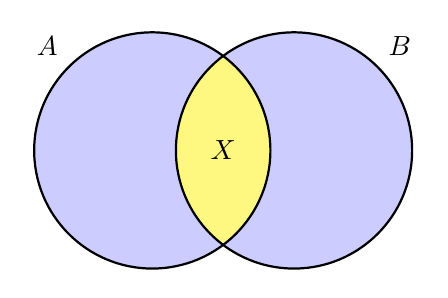
\begin{tikzpicture}[thick, set/.style = {circle, minimum size = 3cm, fill=blue!20}]

        % Set A
        \node[set,label={135:$A$}] (A) at (0,0) {};

        % Set B
        \node[set,label={45:$B$}] (B) at (1.8,0) {};

        % Intersection
        \begin{scope}
            \clip (0,0) circle(1.5cm);
            \clip (1.8,0) circle(1.5cm);
            \fill[yellow!50](0,0) circle(1.5cm);
        \end{scope}

        % Circles outline
        \draw (0,0) circle(1.5cm);
        \draw (1.8,0) circle(1.5cm);

        % Set intersection label
        \node at (0.9,0) {$X$};
    \end{tikzpicture} 
\end{center}

为了证明这个命题,我们引入任意固定元素 $x \in X$。关于它我们知道什么?假设 $X \subseteq A$。符号``$\subseteq$''的定义表明 $X$ 的所有元素都属于 $A$。既然 $x$ 是 $X$ 的元素,那么 $x$ 也属于 $A$。这很方便!类似地,由 $X \subseteq B$ 可得 $x \in B$。综上,我们利用``$\cap$''的定义推知 $x \in A \cap B$。很好!现在将其形式化。

\begin{proof}
    设 $x \in X$ 为任意固定元素。

    假设 $X \subseteq A$,根据 $\subseteq$ 的定义,可得 $x \in A$。

    同理,由 $X \subseteq B$,可得 $x \in B$。

    因为 $x \in A$ 且 $x \in B$,根据 $\cap$ 的定义,这意味着 $x \in A \cap B$。

    综上,对任意 $x \in X$ 均有 $x \in A \cap B$。由于 $x \in X$ 是任意的,因此 $X \subseteq A \cap B$。
\end{proof}

下面看一个稍复杂的例子。

\begin{proposition}
    设 $A$ 和 $B$ 为任意集合。则 $\mathcal{P}(A) \cap \mathcal{P}(B) \subseteq \mathcal{P}(A \cap B)$。
\end{proposition}

这成立吗?回顾 \ref{sec:section3.5} 节习题 \ref{exc:exercises3.5.6} 中的具体示例可知,该命题具有一般性。下面证明其正确性。

\emph{直观理解}:此命题涉及多层次的定义,尤其需注意幂集运算。关键点在于理解 $\mathcal{P}(A)$ 是 $A$ 的所有子集的集合。待证子集关系表明:无论 $\mathcal{P}(A) \cap \mathcal{P}(B)$ 的具体形式如何(稍后分析,但眼下你需要意识到它是一个集合),它都是 $\mathcal{P}(A \cap B)$ 的子集。这一观察将引导后续证明的框架。

无需显式计算 $\mathcal{P}(A) \cap \mathcal{P}(B)$,证明可从``设 $X \in \mathcal{P}(A) \cap \mathcal{P}(B)$ 为任意集合''开始。因为根据``$\subseteq$''的定义,需要证明该集合的任意元素也属于 $\mathcal{P}(A \cap B)$。这确定了证明的\textbf{结构}。

元素 $X \in \mathcal{P}(A) \cap \mathcal{P}(B)$ 是什么?它是集合,且同时属于 $\mathcal{P}(A)$ 和 $\mathcal{P}(B)$。下面直接给出正式证明,但建议你先尝试自行证明。完成后可与下文比较,检验步骤的完整性和表述的清晰性。

\begin{proof}
    设 $X \in \mathcal{P}(A) \cap \mathcal{P}(B)$ 为任意固定集合。

    根据 $\cap$ 的定义,有 $X \in \mathcal{P}(A)$ 且 $X \in \mathcal{P}(B)$。

    因为 $X \in \mathcal{P}(A)$,根据幂集的定义,可知 $X \subseteq A$。

    同理,因为 $X \in \mathcal{P}(B)$ 可知 $X \subseteq B$。

    因为 $X \subseteq A$ 且 $X \subseteq B$,由引理 \ref{lemma3.9.1} 可得 $X \subseteq A \cap B$。

    因为 $X \subseteq A \cap B$,根据幂集的定义,可得 $X \in \mathcal{P}(A \cap B)$。

    由于 $X$ 是任意固定集合,因此可得 $\mathcal{P}(A) \cap \mathcal{P}(B) \subseteq \mathcal{P}(A \cap B)$。
\end{proof}

你的证明与上述一致吗?是否引用了前述引理?或无意中复证了已有结论?请记住:证明的重要价值在于结论的可复用性!虽在证明中复证先前结论无技术错误,但直接引用可节省精力。若解题时产生``似曾相识''的感觉,不妨回溯相关定理或引理,利用已有结论提升效率。


% !TeX root = ../../../book.tex
\subsection{证明``$=$''}

\subsubsection*{双重包含证明}

我们需要再次回顾在集合上下文中``$=$''的定义,因为后续会频繁使用它。

\begin{definition}
    集合 $A$ 和 $B$ 相等,记作 $A = B$,当且仅当 $A \subseteq B$ 且 $B \subseteq A$。
\end{definition}

这一定义完全基于先前定义的``$\subseteq$''(因为``$\supseteq$''的定义等价)。因此,它并非新技术,而是先前技术的重复应用。具体而言,要证明 $A = B$,只需使用上一小节的技术证明 $A \subseteq B$,再证明 $B \subseteq A$。

事实上,这项技术非常常见,因此有专门的名称:\textbf{双重包含}。当证明两个集合彼此是子集并由此得出它们相等时,称为\textbf{双重包含证明}。

\subsubsection*{示例}

让我们看一下双重包含技术的实际应用案例。

\begin{lemma}
    设 $A$ 和 $B$ 为任意集合,则 $A - (A \cap B) = A - B$。
\end{lemma}

\emph{直观理解}:虽然维恩图可以帮助理解这一事实,但它不能替代证明。我们将采用双重包含证明。取元素 $x \in A - (A \cap B)$ 时,可依次应用``$-$''和``$\cap$''的定义,推导出 $x \in A - B$。类似地,取 $y \in A - B$ 时,应用定义可得出 $y \in A - (A \cap B)$。建议读者先尝试自行证明,再参考以下证明过程。

\begin{proof}
    通过双重包含证明 $A - (A \cap B) = A - B$。

    (``$\subseteq$'')设 $x \in A - (A \cap B)$ 为任意固定元素。根据差集定义,$x \in A$ 且 $x \notin A \cap B$。这意味着 $x$ 不可能同时属于 $A$ 和 $B$。已知 $x \in A$,故 $x \notin B$。因此,$x \in A$ 且 $x \notin B$,由差集定义得 $x \in A-B$。这表明 $A - (A \cap B) \subseteq A - B$。

    (``$\supseteq$'')设 $y \in A - B$ 为任意固定元素。根据差集定义,$y \in A$ 且 $y \notin B$。由于 $y \notin B$,$y$ 不可能同时属于 $A$ 和 $B$。由交集定义,$y \notin A \cap B$。结合 $y \in A$ 和 $y \notin A \cap B$,得 $y \in A - (A \cap B)$。这表明 $A - B \subseteq A - (A \cap B)$。

    综上,利用双重包含证明,$A - (A \cap B) = A - B$ 得证。
\end{proof}

纵观上述证明的整体结构,我们看到它分为两部分,因为它是一个双重包含证明。我们\emph{友好地提前}向读者指出了这一点,并将这两个部分明确分开。从技术上讲,忽略这一提示直接深入证明是可行的,但这可能会令读者感到困惑。证明的全部意义在于\emph{使他人信服}你所理解的事实,因此应尽可能让读者轻松理解你的思路。

现在看另一个证明集合相等的例子。这个例子有所不同,因为双重包含的一部分利用了补集操作。作为预习,请思考为何命题 $A \subseteq B$ 与 $\overline{B} \subseteq \overline{A}$ 是\emph{等价的}(假设存在全集 $U$ 满足 $A, B \subseteq U$)。尝试绘制维恩图、举例或直接证明。

\begin{proposition}
    \[\Big\{x \in \mathbb{N} \mid x + \frac{8}{x} \le 6\Big\} = \{2, 3, 4\}\]
\end{proposition}

\begin{proof}
    设 $A = \Big\{x \in \mathbb{N} \mid x + \frac{8}{x} \le 6\Big\}$, $B = \{2, 3, 4\}$。要证明 $A = B$,需要证明 $A \subseteq B$ 且 $B \subseteq A$。

    首先证明 $B \subseteq A$。逐一验证 $B$ 的元素是否满足 $A$ 的不等式:
    \begin{align*}
        2 + \frac{8}{2} &= 6 \le 6 \\
        3 + \frac{8}{3} &= \frac{17}{3} \le 6 \\
        4 + \frac{8}{4} &= 6 \le 6
    \end{align*}
    因为 $2,3,4 \in \mathbb{N}$,我们推导出 $2,3,4 \in A$,从而 $B \subseteq A$。

    接着证明 $A \subseteq B$。我们将证明 $\overline{B} \subseteq \overline{A}$,其中补集以 $\mathbb{N}$ 为全集。也就是说,我们要证明自然数 $1,5,6,7,\dots$ \dotuline{不}属于 $A$。

    为此,验证这些元素均\dotuline{不}满足 $A$ 的不等式定义:

    前两种情况很容易验证:
    \begin{align*}
        1 + \frac{8}{1} &= 9 \nleq 6 \\
        5 + \frac{8}{5} &= \frac{33}{5} \nleq 6
    \end{align*}

    对于其他情况,取任意固定元素 $x \in \mathbb{N}$ 且 $x \ge 6$,有 $x + \frac{8}{x} \ge 6 + \frac{8}{x}$。由于 $\frac{8}{x} > 0$,故 $x + \frac{8}{x} > 6$。

    这表明只有 $2,3,4$ 满足 $A$ 的不等式定义。

    综上,利用双重包含证明,$A = B$ 得证。
\end{proof}

思考为何证明后半部分的方法有效。(这是条件命题的\textbf{逆否}形式,后续章节讨论逻辑时将详细说明。)

让我们来看另一个证明集合相等的例子。这个例子略有不同,因为我们要证明某个集合是空集,为此需要证明它不包含任何元素。

\begin{proposition}
    对于每个 $n \in \mathbb{N}$,定义 $S_n = \mathbb{N}-[n]$。则
    \[\bigcap_{n \in \mathbb{N}}S_n = \varnothing\]
\end{proposition}

如果不理解上面等式的含义,建议尝试几个例子。例如,查看集合 $S_1$、$S_1 \cap S_2$、$S_1 \cap S_2 \cap S_3$ 的元素等等。可以先找出 $\bigcap_{n \in \mathbb{N}}S_n$ 的候选元素,再解释为什么它不属于该集合。之后尝试写出一个正式的证明;可以参考下面的证明过程!

\begin{proof}
    设 $T = \bigcap_{n \in \mathbb{N}}S_n$ 以便后续引用。

    要证明 $T = \varnothing$,需要证明 $T$ 不包含任何元素。注意 $T$ 是多个自然数集合的交集,因此其元素只能是自然数。

    考虑任意固定元素 $x \in \mathbb{N}$,我们需要证明 $x \notin T$。

    已知 $x \in [x] = \{1,2,\dots, X\}$,因此根据``$-$''的定义,$x \notin \mathbb{N}-[x]$。

    根据定义,$T$ 的元素必须属于每个 $\mathbb{N} - [n]$ 形式的集合。我们已经(至少)确定了交集中的一个集合 $\mathbb{N} - [x]$,使得 $x$ 不属于该集合。因此,$x$ 不可能是 $T$ 的元素,因为它不属于所有此类集合,所以 $x \notin T$。

    因为 $x \in \mathbb{N}$ 是任意的,我们证明了 $T$ 的元素中不包含自然数,故 $T$ 为空集。
\end{proof}

\emph{总结}:让我们再解释一下这个证明方法为何有效。我们证明了 $T$ 中没有元素,即 $T \subseteq \varnothing$。这就完成了论证,因为 $\varnothing \subseteq T$ 对任何集合恒成立。因此双重包含论证的条件已满足,可以得出 $T = \varnothing$ 的结论。

让我们再举一个例子。这个例子为我们提供了练习索引集操作的机会,本节习题中还有许多类似问题,我们鼓励你尽可能多尝试解答!

\begin{proposition}
    对于每个 $n \in \mathbb{N}$,定义 $A_n = \{x \in \mathbb{R} \mid 0 \le x < \frac{1}{n}\}$。则
    \[\bigcap_{n \in \mathbb{N}}A_n = \{0\}\]
\end{proposition}

思考上述命题的含义:在数轴上画出 $A_n$ 的图示,交集符号``$\cap$''表示什么?为什么 $0$ 属于该交集?为什么它是\emph{唯一}的元素?

证明的关键在于``$\cap$''的定义,请特别注意\emph{对于每个}这一条件:

\begin{definition}
    由集合 $I$ 索引的一系列集合 $A_i$ 的交集为
    \[\bigcap_{i \in I} A_i = \{x \in U \mid x \in A_i \text{\ 对于每个\ } i \in I\}\]
    其中我们假设存在集合 $U$ 满足对于每个 $i \in I, A_i \subseteq U$。
\end{definition}

请牢记:索引交集由属于所有成分集合的元素构成。因此在证明中,我们需要说明:
\begin{enumerate}[label=(\arabic*)]
    \item $0$ 确实是所有 $A_n$ 集合的元素。
    \item 不存在其他实数满足此性质,即对于任意非零实数,总存在某个 $A_n$ 不包含该数。
\end{enumerate} 

\begin{proof}
    首先,我们来证明
    \[\{0\} \subseteq \bigcap_{n \in \mathbb{N}}A_n\]

    这需要证明对于每个 $n \in \mathbb{N}, 0 \in A_n$。

    设 $n \in \mathbb{N}$ 为任意固定元素。注意,不等式 $0 \le 0 \le \frac{1}{n}$ 必然成立。

    (注:可能有人会担忧,因为``在极限内'' $0$ 是否``同时''小于每个分数 $\frac{1}{n}$,但这不是重点!正确的思路是:$0 \in A_1$ 吗?是的,因为 $0 \le 0 < 1$。$0 \in A_2$ 吗?是的,因为 $0 \le 0 < \frac{1}{2}$。$0 \in A_3$ 吗?是的,因为 $0 \le 0 < \frac{1}{3}$。依此类推。该不等式对于每个 $n \in N$ 均成立,所以 $0$ 是每个此类集合的元素。如果你不担心这一点,可跳过此备注,继续前进!)

    因此,对于每个 $n \in \mathbb{N}, 0 \in A_n$,所以根据 ``$\cap$'' 的定义,$\displaystyle{0 \in \bigcap_{n \in \mathbb{N}} A_n}$。这就证明了 $\displaystyle{\{0\} \subseteq \bigcap_{n \in \mathbb{N}} A_n}$。

    接着,我们来证明
    \[\bigcap_{n \in \mathbb{N}}A_n \subseteq \{0\}\]

    考虑在全集 $\mathbb{R}$ 下这些集合的\dotuline{补集}。具体来说,我们将证明
    \[\overline{\{0\}} \subseteq \overline{\bigcap_{n \in \mathbb{N}}A_n}\]

    这意味着我们要证明每个非零实数\dotuline{不属于}某个 $A_n$。

    设 $x \in \mathbb{R}$ 为任意固定元素,且 $x \ne 0$。也就是说,要么 $x > 0$ 要么 $x < 0$。接下来分两种情况讨论:

    \begin{itemize}
        \item 情况 1:假设 $x > 0$。考虑实数 $\frac{1}{x} \in \mathbb{R}$。由于 $\mathbb{R}$ 中的自然数集无上界,因此存在 $M \in \mathbb{N}$ 满足 $M > \frac{1}{x}$。
        
        (注意:思考为什么会这样。我们尚未\dotuline{证明} $\mathbb{N}$ 是无限的,即数字沿着实数轴``永远延续下去'',但我们希望这些想法对你来说直观且合理。)

        取 $M \in \mathbb{N}$ 且 $M > \frac{1}{x}$。由于 $x > 0$,不等式两边同时乘以 $x$;由于 $M > 0$(因此 $\frac{1}{M} > 0$),不等式两边再次乘以 $\frac{1}{M}$。由此可得 $x > \frac{1}{M}$。由于 $A_M$ 要求 $-\frac{1}{M} < x < \frac{1}{M}$,因此 $x \ne A_M$。

        由于 $x \notin A_M$,所以 $x$ 肯定不是所有此类集合的元素。因此
        \[x \notin \bigcap_{n \in \mathbb{N}} A_n\]

        \item 情况 2:假设 $x < 0$。考虑 $-x > 0$。采用与上面相同的逻辑,必然存在 $M \in \mathbb{N}$ 满足 $M > \frac{1}{-x} = -\frac{1}{x}$。整理不等式可得 $x < -\frac{1}{M}$。所以 $x \notin A_M$,因此 
        \[x \notin \bigcap_{n \in \mathbb{N}} A_n\]
    \end{itemize}

    综上,我们已经证明,任意 $x \in \mathbb{R}$ 且 $x \ne 0$ 不属于至少一个 $A_n$,因此任何这样的 $x$ 都不是它们交集的元素。因此,由双重包含论证可得:
    \[\{0\} = \bigcap_{n \in \mathbb{N}} A_n\]
\end{proof}

该证明具有一定难度,建议反复阅读确保理解每个步骤。特别留意选择 $M \in \mathbb{N}$ 且满足 $M > \frac{1}{x}$ 的动机:这并凭借直觉神奇偶得,而是从目标 $x > \frac{1}{M}$ 反推不等式得到的。


% !TeX root = ../../../book.tex
\subsection{证伪}

\subsubsection*{举个例子}

考虑如下命题:
\begin{center}
    对于任意集合 $F, G, H$,如果 $F \subseteq G \cup H$,则要么 $F \subseteq G$ 要么 $F \subseteq H$。
\end{center}

这种说法成立吗?如果成立,我们该如何证明呢?我们取任意固定元素 $x \in F$。由于 $F \subseteq G \cup H$,这告诉我们 $x \in G \cup H$。 相应地,$x \in G$ 或 $x \in H$。这都没错吧?我们的证明完成了吗?

我们希望你能看出来这是行不通的!特别是,我们最后还没有满足 ``$\subseteq$'' 的定义。如果我们的目标是证明 ``$F \subseteq G$ 或 $F \subseteq H$'',那么我们应该得出结论,其中一个或另一个成立:即 $F$ 的\emph{每个}元素都是 $G$ 的元素,或者 $F$ 的\emph{每个}元素都是 $H$ 的元素。

我们发现 $F$ 的每个元素本身要么是 $G$ 的元素,要么是 $H$ 的元素,但我们不能确定 $F$ 的所有元素都是 $G$ 的元素或都是 $H$ 的元素。再次通读最后两段,以确保你跟上了逻辑。可能很容易为这个命题写出一个``证据'',却没有意识到你迈出了错误的一步!

\subsubsection*{定位错误}

这种对错误的识别是我们要发展的技能之一,它将在多个方面提供帮助。你会注意到,许多练习(到目前为止有一些,但随着我们继续深入,会有更多)要求你找出某些主张``证明''中的缺陷。通过指出存在缺陷,从而帮助你获得正确的证明(或多个证明,视情况而定)。阅读在逻辑、事实和清晰度上有误的证明是一项基本技能。更重要的是,仔细阅读别人的成果必然会让你成为一个对自己的成果更加挑剔的读者,并且会帮助你发现像前面段落中那样的潜在错误。如果你没有抓住它,请不要担心;既然你已经看到了它,你将来就会留意类似的错误!正如我们所说,这项技能是不断发展起来的,到读完本书时,你将成为数学证明的出色读者和作者。

\subsubsection*{反例}

那么,现在我们该怎么办?我们刚刚意识到我们上面的``证明''不起作用。这是否意味着该说法实际上是错误的?实际上,这一切意味着(到目前为止)我们的证明尝试失败了。也许其他一些逻辑路线会神奇地把我们带到难以捉摸的结论。

或者,也许这个说法确实是错误的。我们怎样才能证明这一点?考虑一下该命题的逻辑形式:它说某些陈述对于任意集合 $F,G,H$ 都成立。它说假设 $F \subseteq G \cup H$ 总是必然意味着 $F \subseteq G$ 或 $F \subseteq H$。要证明这并不总是成立,我们只需要找到所谓的\textbf{反例}即可。

我们将在下一章形式化逻辑时再次讨论所有这些想法,但现在你需要知道的是:\textbf{反例}是一个具体的、详细的、描述性的例子,它说明了关于``每个……''或``任意……''或``皆可能……''实际上并\emph{不}适用于所有情况。反例相当于通过展示该类中\emph{不具有}该属性的一个对象来\textbf{反驳}整个类对象具有某种属性的陈述。

\subsubsection*{示例}

让我们看一下寻找和陈述反例的过程如何解决我们上面的例子。\\

\begin{example}
    对于任意集合 $F, G, H$,如果 $F \subseteq G \cup H$,则要么 $F \subseteq G$ 要么 $F \subseteq H$。
\end{example}

这个命题应该适用于任意集合 $F,G,H$,因此当我们描述反例时,我们最好\emph{准确地}描述这三个集合是什么。我们不能只是解释解决这个问题的方法并讨论如何可能存在具有特定属性的三个集合。我们必须通过明确定义它们来告诉读者它们到底是什么。这就是我们反驳这一主张的第一行,但我们不能直接跳到这一点,因为我们还不知道如何定义它们!

这就是工作或乐趣所在:我们需要尝试这些集合所需的属性来帮助我们想出一个例子。回想一下,我们希望这些集合满足某些属性:我们应该确保假设 $F \subseteq G \cup H$ 成立,但我们希望结论 --- $F \subseteq G$ 或 $F \subseteq H$ --- 为假。

这是意味着什么呢?好吧,我们认为你会同意,从逻辑上讲,该陈述的``相反''或``否定''是 ``$F \nsubseteq G$'' 和 ``$F \nsubseteq H$''。(\textbf{逻辑否定}的概念将在下一章中再次出现;目前,我们认为你可以通过应用指导日常生活的逻辑原则来理解它。很快,我们将正式化这一想法。)

我们现在有一个具体的目标:找到满足以下所有三个条件的三个集合 $F,G,H$:

\begin{align*}
    F &\subseteq G \cup H \\
    F &\nsubseteq G \\
    F &\nsubseteq H \\
\end{align*}

接下来需要考虑的一件事是 ``$\nsubseteq$'' 的含义。我们有 ``$\subseteq$'' 的定义,那么它的``相反''或``否定''是什么?为了使 $F \subseteq G$ 成立,我们要求 $F$ 的每个元素也是 $G$ 的元素;因此,如果不成立,那么 $F$ 中至少有一个元素不是 $G$ 的元素。同理也适用于 $F \nsubseteq H$。现在,我们可以通过应用定义以一种有用的方式重申我们的目标:

\begin{align*}
    &F \text{的每个元素都是} G \text{的元素或} H \text{的元素} \\
    &F \text{中至少有一个元素不是} G \text{的元素} \\
    &F \text{中至少有一个元素不是} H \text{的元素} \\
\end{align*}
这对于最终找到我们的反例非常有帮助!我们总结了声明的所有基本部分,并以更直观的方式重述了这些属性。剩下的工作就是在草稿纸上写写画画,看看我们能想出什么。一种方法是为 $F, G$ 和 $H$ 及其潜在的``重叠''绘制一种``空''维恩图,然后填充足够的元素以满足上述三个属性。

第一个条件要求集合 $F$ 完全``位于'' $G$ 和 $H$ 之内;但是,第二个和第三个条件要求存在 $F$ 的两个元素,其中一个不是 $G$ 的元素,另一个不是 $H$ 的元素。这就是我们要做的!你可能会说这是一个简单的例子,但我们说这是一个\emph{有效的}例子。现在让我们开始写下我们的反驳:

\begin{proof}
    下面声明为假:
    \begin{center}
        对于任意集合 $F, G, H$,如果 $F \subseteq G \cup H$,则要么 $F \subseteq G$ 要么 $F \subseteq H$。
    \end{center}
    我们将用反例来反驳该观点。

    定义 $F = \{1, 2\}, G = \{1\}, H = \{2\}$。

    请注意 $G \cup H = \{1, 2\}$。由于 $F = G \cup H$,那么当然 $F \subseteq G \cup H$。因此,该主张的假设成立。

    然而,请注意 $2 \in F$ 但 $2 \notin G$。因此,$F \nsubseteq G$。

    同样,请注意 $1 \in F$ 但 $1 \notin H$。因此,$F \nsubseteq H$。

    因此,该主张为假。
\end{proof}

该示例的一个重要教训如下:

\begin{center}
    寻找反例不一定是最有趣或最复杂的,你也不需要以某种方式描述所有可能的反例。我们只需要找到一个反例,我们需要看看它是如何运作的。
\end{center}

就是这样!这正是我们在上面的证明中所做的:我们定义了所有重要的对象(三个集合 $F,G,H$),然后指出并描述了它们具有的所有相关属性。我们并没有让读者检查反例是否有效;我们向他们展示了细节。我们并没有争论宇宙中某个地方存在这样的集合;我们只是认为宇宙中存在这样的集合。我们明确地定义了它们。

这很重要,我们希望你的反例具有与我们上面类似的证明结构。当你尝试给出反例时,大部分工作将在证明开始之前``在幕后''进行。不过,一旦你找到了反例,就像我们一样把它写出来。


% !TeX root = ../../../book.tex
\subsection{习题}

\subsubsection*{温故知新}

以口头或书面的形式简要回答以下问题。这些问题全都基于你刚刚阅读的内容,所以如果忘记了具体的定义、概念或示例,可以回去重读相关部分。确保在继续学习之前能够自信地回答这些问题,这将有助于你的理解和记忆!

\begin{enumerate}[label=(\arabic*)]
    \item $\subseteq$ 的定义是什么?我们如何用它来证明 $A \subseteq B$?
    \item 两个集合相等意味着什么?
    \item 什么是\emph{双重包含}证明?
    \item 什么是反例?
    \item 假设 $A,B,U$ 是集合,且 $A,B \subseteq U$。为什么我们可以通过证明 $\overline{B} \subseteq \overline{A}$ 来证明 $A \subseteq B$ 呢?尝试说服朋友相信这是一种有效的技术。
\end{enumerate}

\subsubsection*{小试牛刀}

尝试回答以下问题。这些题目要求你实际动笔写下答案,或(对朋友/同学)口头陈述答案。目的是帮助你练习使用新的概念、定义和符号。题目都比较简单,确保能够解决这些问题将对你大有帮助!

\begin{enumerate}[label=(\arabic*)]
    \item 首先,\textbf{证明}如下声明:
        \begin{center}
            对于任意集合 $A,B,C$,子集关系 $A - (B - C) \subseteq (A - B) \cup C$ 成立。
        \end{center}
        接着,找到这些集合实际上总是\emph{相等}这一主张的\emph{反例}。
    \item 假设 $A,B,C$ 是集合并且 $A \subseteq B$。证明 $A \times C \subseteq B \times C$。
    \item 假设 $A \subseteq C$ 且 $B \subseteq D$。证明 $A \times C \subseteq B \times C$。
    \item 设 $A = \{x \in \mathbb{R} \mid x^2 > 2x + 8\}$ 且 $B = \{x \in \mathbb{R} \mid x > 4\}$。对于以下每个主张,要么证明它是正确的,要么提供反例来证明它是错误的。
        \begin{enumerate}[label=(\alph*)]
            \item $A \subseteq B$
            \item $B \subseteq A$
        \end{enumerate}
    \item 设 $A, B, U$ 为集合,且 $A, B \subseteq U$。通过\emph{双包含论证}证明 $A - B = A \cap \overline{B}$。
    \item 令 $S = \{x \in \mathbb{R} \mid -2 < x < 5\}$ 且 $T = \{x \in \mathbb{R} \mid -4 \le x \le 3\}$。在 $\mathbb{R}$ 作为全集的情况下,$S \cap \overline{T}$ 是什么?找到一个集合,然后使用双包含论证证明它是正确的。
    \item \textbf{证明}以下断言:如果 $A \subseteq B$,则 $\mathcal{P}(A) \subseteq \mathcal{P}(B)$。\label{exc:exercises3.9.7}
    \item 对于每个 $n \in \mathbb{N}$ 令 $S_n = \{x \in \mathbb{R} \mid -\frac{1}{n} < x < \frac{1}{n}\}$。证明
        \[\bigcap_{n \in \mathbb{N}}S_n = \{0\}\]
    \item 设 $I = \{x \in \mathbb{R} \mid 0 < x < 1\}$。对于每个 $x \in I$,定义 $S_x = \{y \in \mathbb{R} \mid x < y < x + 1\}$。 证明
        \[\bigcup_{x \in I}S_x = \{z \in \mathbb{R} \mid 0 < z < 2\}\]
    \item 对于每个 $n \in \mathbb{N}$,定义集合 $A_n$ 和 $B_n$
        \begin{align*}
            A_n &= \Big\{x \in \mathbb{R} \mid 0 ≤ x < \frac{n - 1}{n}\Big\} \\
            B_n &= \Big\{y \in \mathbb{R} \mid -\frac{1}{n} < y < 1\Big\}
        \end{align*}
        通过双重包含论证\textbf{证明}以下集合相等:
        \[\bigcup_{n \in \mathbb{N}}A_n = \bigcap_{n \in \mathbb{N}}B_n\]
\end{enumerate}


\newpage
% !TeX root = ../../../book.tex
\section{总结}

本章初步探索了抽象概念与结果。我们引入了\textbf{集合}的概念,并通过实例帮助读者建立理解。重点讨论了\textbf{元素}与\textbf{子集}的核心关系,并强调区分二者至关重要(``口袋类比''可辅助记忆)。同时介绍了包括集合构造符在内的符号体系。随着数学抽象程度的加深,规范使用形式化符号对准确表达思想将变得至关重要。核心概念\emph{幂集}将\emph{元素}与\emph{子集}关系紧密联系。

关于集合运算的讨论揭示了组合集合生成新集合的方法,这些操作贯穿全书。我们还演示了如何通过\emph{索引}处理多个集合,这让我们能够仅用基础定义与符号简洁地写出多个集合的并集。这些思想将在后续内容中反复出现,因此设置了大量相关练习,建议读者尽可能尝试解决!

我们还介绍了集合论的核心证明技术——\textbf{双向包含论证}。这一基础方法将频繁出现于本课程及其他研究领域。

本章还探讨了抽象集合论中的若干深刻洞见。\emph{罗素悖论}揭示了``所有集合的集合''不存在;而自然数的集合论定义虽具理论价值,实践中我们仍将沿用对 $\mathbb{N}$ 的直观理解。希望这些讨论兼具趣味性与启发性。


\newpage
% !TeX root = ../../../book.tex
\section{本章习题}

本节习题涵盖本章全部内容,并涉及先前知识点及部分数学假设。我们不要求你解答\textbf{所有}题目,但解决得越多,收获越大!请牢记:真正\emph{掌握}数学必须亲自\emph{实践}。尝试动手解题,仔细阅读并思考题意。撰写证明并与朋友讨论,检验其说服力。持续练习如何清晰、准确、有条理地\emph{书写}思路。完成证明后要反复修改以臻完善。最重要的是,坚持\emph{钻研}数学!

标有 $\blacktriangleright$ 的简答题只需解释或陈述答案,无需严格证明。

特别具有挑战性的问题标记为 $\bigstar$。

\begin{exercise}
    $\blacktriangleright$ 请判断以下关于元素和子集的陈述是是否成立,并准备好向持怀疑态度的朋友解释你的结论!
    本题中统一使用如下定义:
    \begin{align*}
        A &= \{x \in \mathbb{Z} \mid -3 \le x \le 3\} \\
        B &= \{y \in \mathbb{Z} \mid -5 < y < 6\} \\
        C &= \{x \in \mathbb{R} \mid x^2 \ge 9\} \\
	    D &= \{x \in \mathbb{R} \mid x < -3\} \\
        E &= \{n \in \mathbb{N} \mid n \text{\ 为偶数} \}
    \end{align*}
    \begin{tasks}(2)
        \task $A \subseteq B$
        \task $C \cap D = \varnothing$
        \task $4 \in E \cap B$
        \task $\{4\} \subseteq A \cap E$
        \task $10 \in C - D$
        \task $A \cup B \supseteq C$
        \task $3 \in A \cap C$
        \task $0 \in (A - B) \cup D$
        \task $E \cap C \subseteq \mathbb{Z}$
        \task $0 \notin B - C$
    \end{tasks}
\end{exercise}

\begin{exercise}
    $\blacktriangleright$ 设 $m, n \in \mathbb{N}$,且 $m \le n$。请解释为什么 $\mathcal{P}([m]) \subseteq \mathcal{P}([n])$。
\end{exercise}

\begin{exercise}
    回顾 \ref{sec:section3.9} 节的问题 \ref{exc:exercises3.9.7}。我们已证明,若 $A \subseteq B$,则必有 $\mathcal{P}(A) \subseteq \mathcal{P}(B)$。请仔细阅读该证明并理解其细节。

    这种说法``反过来''是否成立?即假设 $\mathcal{P}(A) \subseteq \mathcal{P}(B)$,能否证明 $A \subseteq B$ 也成立?若不能,请构造反例。
\end{exercise}

\begin{exercise}
    用``集合构建符''重写以下定义。如果可能的话,直接列举集合元素;否则说明原因并给出三个示例元素。
    \begin{enumerate}[label=(\alph*)]
        \item 设 $A$ 为平方小于 $39$ 的所有自然数的集合。
        \item 设 $B$ 为方程 $x^2 - 3x - 10 = 0$ 所有实根的集合。
        \item 设 $C$ 为和为非负数的整数对的集合。
        \item 设 $D$ 为实数对的集合,其中第一个坐标为正,第二个坐标为负,且两个坐标和为正。
    \end{enumerate}
\end{exercise}

\begin{exercise}
    定义如下集合:
    \begin{align*}
        A &= \{x \in \mathbb{R} \mid x^2 - x - 12 < 0 \} \\
        B &= \{y \in \mathbb{R} \mid -3 < y < 4\}
    \end{align*}
    证明 $A = B$。
\end{exercise}

\begin{exercise}
    设 $X$ 为某学校全体学生的集合。
    \begin{itemize}
        \item 定义属性 $P(x)$,使得 $A := \{x \in X \mid P(x)\}$ 是 $X$ 的非空真子集。
        \item 定义属性 $Q(x)$,使得 $B := \{x \in X \mid Q(x)\}$ 是 $A$ 的非空真子集。
    \end{itemize}
\end{exercise}

\begin{exercise}
    设 $A, B, C$ 为集合,且 $A \subseteq C$, $B \subseteq C$。
    \begin{enumerate}[label=(\alph*)]
        \item 绘制集合 $\overline{A} \cap \overline{B}$ 和 $\overline{(A \cap B)}$ 的维恩图。
        \item 证明 $\overline{A} \cap \overline{B} \subseteq \overline{(A \cap B)}$。
        \item 构造集合 $A,B,C$,使得 $\overline{A} \cap \overline{B} \subset \overline{(A \cap B)}$。
        \item 构造集合 $A,B,C$,使得 $\overline{A} \cap \overline{B} = \overline{(A \cap B)}$。
    \end{enumerate}
\end{exercise}

\begin{exercise}
    令 $S = \{(m, n) \in \mathbb{Z} \times \mathbb{Z} \mid m = n^2\}$。$S$ 与集合 $T = \{(m, n) \in \mathbb{Z} \times \mathbb{Z} \mid n = m^2\}$ 的关系如何?如果一个是另一个的子集,请给出证明。如果不是,请给出反例。
\end{exercise}

\begin{exercise}
    令 $(a,b)$ 为笛卡尔平面上的一点,即 $(a,b) \in \mathbb{R} \times \mathbb{R}$。设 $\varepsilon$(希腊字母 \emph{epsilon})为非负实数,即 $\varepsilon \in \mathbb{R}$ 且 $\varepsilon \ge 0$。\\
    设 $C_{(a,b),\varepsilon}$ 为``接近'' $(a, b)$ 的点集,定义如下:
    \[C_{(a,b),\varepsilon} = \Big\{(x, y) \in \mathbb{R} \times \mathbb{R} \mid \sqrt{(x - a)^2 + (y - b)^2} < \varepsilon\Big\}\]
    \begin{enumerate}
        \item 给出集合 $C_{(a,b),\varepsilon}$ 的几何描述。
        \begin{itemize}
            \item 当我们改变 $a$ 和 $b$ 时,集合会如何变化?
            \item 当我们改变 $\varepsilon$ 时,集合会如何变化?
        \end{itemize}
        \item $C_{(0,0),1} \cap C_{(0,0),2}$ 是什么?
        \item $C_{(0,0),1} \cup C_{(0,0),2}$ 是什么?
        \item $C_{(0,0),1} \cap C_{(2,2),1}$ 是什么?
    \end{enumerate}
\end{exercise}

\begin{exercise}
    考虑如下(错误)命题:
    \[\bigcup_{n \in \mathbb{N}}\mathcal{P}([n]) = \mathcal{P}(\mathbb{N})\]
    \begin{enumerate}[label=(\alph*)]
        \item 下面的``证明''有什么问题?指出错误并解释其如何破坏了``证明''。
            \begin{spoof}
                首先证明 $\displaystyle{\bigcup_{n \in \mathbb{N}}\mathcal{P}([n]) \subseteq \mathcal{P}(\mathbb{N})}$。

                考虑左侧并集的任意元素 $X$。

                根据索引并集的定义,我们知道存在 $k \in \mathbb{N}$ 使得 $X \subseteq [k]$。

                由于 $[k] \subseteq \mathbb{N}$ 且 $X \subseteq [k]$,我们可以推断出 $X \subseteq \mathbb{N}$。

                因此 $X \in \mathcal{P}(\mathbb{N})$。

                接着证明 $\displaystyle{\bigcup_{n \in \mathbb{N}}\mathcal{P}([n]) \supseteq \mathcal{P}(\mathbb{N})}$。

                考虑任意元素 $Y \subseteq \mathcal{P}(\mathbb{N})$。

                由于 $Y$ 是自然数的子集,我们知道存在 $\ell \in \mathbb{N}$ 使得 $Y \subseteq [\ell]$。

                根据索引并集的定义,可得 $\displaystyle{Y \in \bigcup_{n \in \mathbb{N}}\mathcal{P}([n])}$。

                由于我们已经证明了 $\subseteq$ 和 $\supseteq$,因此两个集合相等。
            \end{spoof}
            $\quad$
        \item 通过构造集合 $S$ 的\textbf{具体}示例反驳该结论,使得
            \[S \in \mathcal{P}(\mathbb{N}) \qquad \text{且} \qquad S \notin \bigcup_{n \in \mathbb{N}}\mathcal{P}([n])\]
    \end{enumerate}
\end{exercise}

\begin{exercise}
    设 $A = [3] \times [4]$。(注意 $[n] = \{1, 2, 3, \dots , n\}$。)\\
    设 $B = \{(x, y) \in \mathbb{Z} \times \mathbb{Z} \mid 0 \le 3x - y + 1 \le 9\}$。
    \begin{enumerate}[label=(\alph*)]
        \item \textbf{证明} $A \subseteq B$。
        \item $A = B$ 吗?\textbf{证明}你的结论并说明原因。
    \end{enumerate}
\end{exercise}

\begin{exercise}
    令 $n \in \mathbb{N}$ 为固定自然数。设 $S = [n] \times [n]$。设 $T$ 为集合
    \[T =\Big\{(x, y) \in \mathbb{Z} \times \mathbb{Z} \mid 0 \le nx + y - (n + 1) \le n^2 - 1\Big\}\]
    证明 $S \subseteq T$ 但 $S \ne T$。
\end{exercise}

\begin{exercise}
    设 $A$ 和 $B$ 为集合。
    \begin{enumerate}[label=(\alph*)]
        \item \textbf{证明} 
        \[\mathcal{P}(A) \cup \mathcal{P}(B) \subseteq \mathcal{P}(A \cup B)\]
        \item 给出 $A$ 和 $B$ 的\textbf{明确}示例,使得 (a) 中的包含是\textbf{严格包含}。
    \end{enumerate}
\end{exercise}

\begin{exercise}
    设 $S$ 和 $T$ 为集合,且它们的本身也是集合。假设 $S \subseteq T$,\textbf{证明} 
    \[\bigcup_{X \in S} X \subseteq \bigcup_{Y \in T} Y\]
\end{exercise}

\begin{exercise}
    设 $A, B, C, D$ 为集合。
    \begin{enumerate}[label=(\alph*)]
        \item \textbf{证明} 
        \[(A \times B) \cup (C \times D) \subseteq (A \cup C) \times (B \cup D)\]
        \item 给出 $A,B,C,D$ 的\textbf{明确}示例,使得 (a) 中的包含是\textbf{严格包含}。
    \end{enumerate}
\end{exercise}

\begin{exercise}
    设 $A, B, C$ 为集合。证明
    \begin{align*}
        A \times (B \cap C) &= (A \times B) \cap (A \times C) \\
        A \times (B - C) &= (A \times B) - (A \times C)
    \end{align*}
\end{exercise}

\begin{exercise}\label{exc:exercises3.11.17} 
    设 $X,Y,Z$ 为集合。证明 $(X \cup Y ) - Z \subseteq X \cup (Y - Z)$,但两者\emph{不一定}相等。
\end{exercise}

\begin{exercise}
    找出集合 $S$ 的示例,使得 $S \in \mathcal{P}(\mathbb{N})$ 且 $S$ 恰好拥有 $4$ 个元素。
    接着找出集合 $T$ 的示例,使得 $T \subseteq \mathcal{P}(\mathbb{N})$ 且 $T$ 恰好拥有 $4$ 个元素。
\end{exercise}

\begin{exercise}
    给出集合 $R,S,T$ 的示例,使得 $R \in S$,$S \in T$,$R \subseteq T$,$R \notin T$。
\end{exercise}

\begin{exercise}
    确定下列集合是什么,并证明你的结论。
    \[\bigcap_{n \in \mathbb{N}}[n] \qquad \text{和} \qquad \bigcup_{n \in \mathbb{N}}[n]\]
\end{exercise}

\begin{exercise}
    设 $I = \{-1, 0, 1\}$。对于每个 $i \in I$,定义 $A_i = \{i - 2, i - 1, i, i + 1, i + 2\}$ 和 $B_i = \{-2i, -i, i, 2i\}$。
    \begin{enumerate}[label=(\alph*)]
        \item 写出 $\displaystyle{\bigcup_{i \in I}A_i}$ 的元素。
        \item 写出 $\displaystyle{\bigcap_{i \in I}A_i}$ 的元素。
        \item 写出 $\displaystyle{\bigcup_{i \in I}B_i}$ 的元素。
        \item 写出 $\displaystyle{\bigcap_{i \in I}B_i}$ 的元素。
        \item 利用上述答案,写出 $\displaystyle{\Big(\bigcup_{i \in I}A_i\Big) - \Big(\bigcup_{i \in I}B_i\Big)}$ 的元素。
        \item 利用上述答案,写出 $\displaystyle{\Big(\bigcap_{i \in I}A_i\Big) - \Big(\bigcap_{i \in I}B_i\Big)}$ 的元素。
        \item 写出 $\displaystyle{\bigcup_{i \in I}(A_i - B_i)}$ 的元素。与 (e) 的答案有何不同?
        \item 写出 $\displaystyle{\bigcap_{i \in I}(A_i - B_i)}$ 的元素。与 (f) 的答案有何不同?
    \end{enumerate}
\end{exercise}

\begin{exercise}\label{exc:exercises3.11.22} 
    在这道题中,我们要``证明''负整数的存在性!我们说``证明''是因为需要完成后续学习才会完全理解这一点,但请相信,这就是我们正在做的事。因此,不能\textbf{假设}存在任何严格小于 $0$ 的整数,故代数步骤(尤其是 (d) 部分)不应涉及可能为负的项。也就是说,若考虑方程
    \[x + y = x + z\]
    我们\textbf{可以}通过两边同时减去 $x$ 推导出 $y = z$,因为 $x - x = 0$。但若考虑方程
    \[x + y = z + w\]
    我们\textbf{不能}推导出 $x - z = w - y$。因为若 $y > w$,则 $w - y$ 在上下文中可能不存在……\\
    \\
    设 $P = \mathbb{N} \times \mathbb{N}$。定义集合 $R$ 为
    \[R = \big\{\big((a, b),(c, d)\big) \in P \times P \mid a + d = b + c \big\}\]
    \begin{enumerate}[label=(\alph*)]
        \item 找出三个不同的 $(c, d)$ 对,使得 $\big((1, 4),(c, d)\big) \in R$。
        \item 设 $(a, b) \in P$。证明 $\big((a, b),(a, b)\big) \in R$。
        \item 设 $\big((a, b),(c, d)\big) \in R$。证明 $\big((c, d),(a, b)\big) \in R$。
        \item 假设 $\big((a, b),(c, d)\big) \in R$ 且 $\big((c, d),(e, f)\big) \in R$。证明 $\big((a, b),(e, f)\big) \in R$。
    \end{enumerate}
\end{exercise}

\newpage
% !TeX root = ../../../book.tex
\section{展望}

现在我们已经介绍了集合,定义了它们,看过了许多示例,并讨论了集合运算以及如何操作集合,现在是时候转向逻辑了。我们已经预览了一些重要的逻辑思想,特别是在第 \ref{sec:section3.9} 节中关于如何撰写集合\textbf{证明}的内容。在下一章中,我们将使所有这些逻辑思想更加正式、明确和严格。我们将开发一些符号和语法,帮助我们更准确、更简洁地表达逻辑思想。我们将使用这些符号和语法以通用语言的形式表达我们的数学思想,并与他人交流我们的想法。简而言之,我们将能够自信地谈论和书写数学!